\documentclass[a4paper,10pt]{scrartcl}
\usepackage[utf8]{inputenc}
\usepackage[T1]{fontenc}
\usepackage{booktabs}
\usepackage{import}
\usepackage{xspace}
\usepackage{enumitem}
\usepackage{cite}
\usepackage{graphicx}
\usepackage{tikz}
\usepackage{wrapfig}
\usepackage{tikz-uml}
\usepackage{gantt}
\usepackage{pdflscape}
\usetikzlibrary{arrows}
\usetikzlibrary{fit}
\usetikzlibrary{calc}
\usepackage{float}
\usepackage{amssymb}
\usepackage{listings}
\usepackage[section]{placeins} % don't move figures beyond the next section heading

% this is needed for forms and links within the text
\usepackage{hyperref}

% Variables
\newcommand{\authorName}{
   Mohammed~Abu~Jayyab,
   Niklas~Baumstark,
   Tobias~Gräf,
   Amrei~Loose,
   Christoph~Michel,
}
\newcommand{\authorNameEmph}{
   Mohammed~Abu~Jayyab,
   Niklas~Baumstark,
   \textbf{Tobias~Gräf},
   Christoph~Michel,
   Amrei~Loose,
}

\newcommand{\dateFirstVersion}{\today}
\newcommand{\customer}{Karlsruhe Institute of Technology}
\newcommand{\contractor}{A company}
\newcommand{\projectName}{Broadcast Encryption\xspace}

\newcommand{\doctitle}{\projectName (Design document)}
\title{\doctitle}
\author{\authorName}
\date{\today}

% less margin
\usepackage[margin=2.5cm]{geometry}

% horizontal line
\newcommand{\HRule}{\rule{\linewidth}{0.5mm}}

% more beautiful lists
\setlist{noitemsep}
\renewcommand{\labelitemi}{$\bullet$}
\renewcommand{\labelitemii}{$\diamond$}

% create a shorter version for tables
\newcommand\addrow[2]{#1 &#2\\ }
\newcommand\addheading[2]{\textbf{\sffamily #1} &\textbf{\sffamily #2}\\ \hline}
\newcommand\tabularhead{\begin{tabular}{lp{13cm}}
\hline
}

\newcommand\addmulrow[2]{ \begin{minipage}[t][][t]{2.5cm}#1\end{minipage}%
   &\begin{minipage}[t][][t]{8cm}
    \begin{enumerate} #2   \end{enumerate}
    \end{minipage}\\ }

\newenvironment{usecase}{\tabularhead}
{\hline\end{tabular}}

% a cross
\newcommand\X{$\times$}

% templates and default styles for figures and graphics
\tikzset{>=triangle 45}
\tikzset{font=\sffamily}

\newcommand{\tmpCaption}{}
\newenvironment{illustration}[1]
{
   \renewcommand{\tmpCaption}{#1}
   \begin{figure}[h!]
   \centering
}
{
   \caption{\tmpCaption}
   \end{figure}
}


\begin{document}

\maketitle
  \begin{tabular}[t]{ll}
	Projekt:       & \quad \projektName \\[1.2ex]
	Auftraggeber:  & \quad \auftraggeber\\[1.2ex]
	Auftragnehmer: & \quad \auftragnehmer\\[1.2ex]
  \end{tabular}

\begin{tabular}{|p{3 cm}|p{3 cm}|p{5 cm}|}
\hline
\textbf{Version} & \textbf{Datum} & \textbf{Autor(en)} \\
\hline
\hline
1.0 & 29.04.2012 & \authorName \\
\hline
\end{tabular}

\tableofcontents
\clearpage

\section{Introduction}
%CryptoCast is a piece of software that provides a service to send contents from a central server to a given
%group of recipients. Transmission happens via a unidirectional communication channel like IP multicast.
%The traffic duplication that would be required for commonly used transport protocols is therefore avoided.

%It enables access control through a specific form of encryption that is based on the Naor-Pinkas broadcast
%encryption scheme. The advantage of this scheme is the 

The software CryptoCast will provide a service for sending encrypted data from a server to certain
amount of people.  This will be implemented as an unidirectional connection that makes it possible for the server
to send data without knowing how many people are receiving it and without the amount of traffic caused
by a bidirectional connection.  Also the type of the sent data will not be determined by the software. So it can be
used for all sorts of data exchange. For demonstration purposes we will implement a simple audio or video stream.

The server will be able to register new users and revoke specific persons if they are not allowed to receive the cast anymore. 
The client is an app on an Android smart phone that is used for receiving, decoding and displaying the data. 
The transport between them will be implemented with TCP but that can be replaced by another transport protocoll.

The implemented encryption algorithm will be the one by Moni Naor and Benny Pinkas, but later every other fitting the
interface can be used. This is important because there might be another more effective algorithm that can replace the implemented one.

In our design we will therefore focuse on modularity and encapsulation to enable substitution for parts of the programm without having to 
change a lot of their enviroment.

\section{Structure}
\subsection{Architecture}

We implement a server-client architecture with one central server sending the stream and multiple clients receiving it.

The server will be designed with a three layer architecture, containing layers for presentation, application and data. In our case 
the presentation layer is presented by the shell, the application layer consists of the controller and the data layer contains ServerData and Command. Dividing the server into those layers makes the different parts less complex and it is possible to modify one layer without having to change the others.

\begin{illustration}{3-tier architecture of the server}

\tikzset{
  rect/.style={draw,fill=green!15,minimum height=0.8cm,rectangle},
  box/.style={
    draw=blue!50!white,
    line width=1pt,
    dash pattern=on 1pt off 4pt on 6pt off 4pt,
    inner sep=4mm, rectangle, rounded corners
  },
}

\begin{tikzpicture}[auto,node distance=1.5cm]

\node[rect,minimum width=6cm](shell) {\textbf{Shell}};
\node[rect,minimum width=3cm,xshift=-1.5cm,below of=shell](control) {Controller};;
\node[rect,minimum width=3cm,below of=control](data) {ServerData};
\node[rect,minimum width=2cm,xshift=2cm, right of=data](cmd) {Command};

\draw [<->]  (shell.south) --  (control.north)
;
\draw [->]  (shell.south) --  (cmd.north)
  ;
\draw [->]  (control.south) --  (data.north)
  ;

\end{tikzpicture}

\end{illustration}

\section{Package description}

\subsection{Package \lstinline!cryptocast.comm!}
This package provides functionality related to communication between the different layers
 of the network protocol and to the communication between the server and clients. This includes
 the management of file and socket streams and abstractions of the multi-client unidirectional
 streams that represent the core of this project.
 Useful abstractions for layered protocols are also included.

\noindent\begin{minipage}[t]{5cm}
\vspace{0.3em}
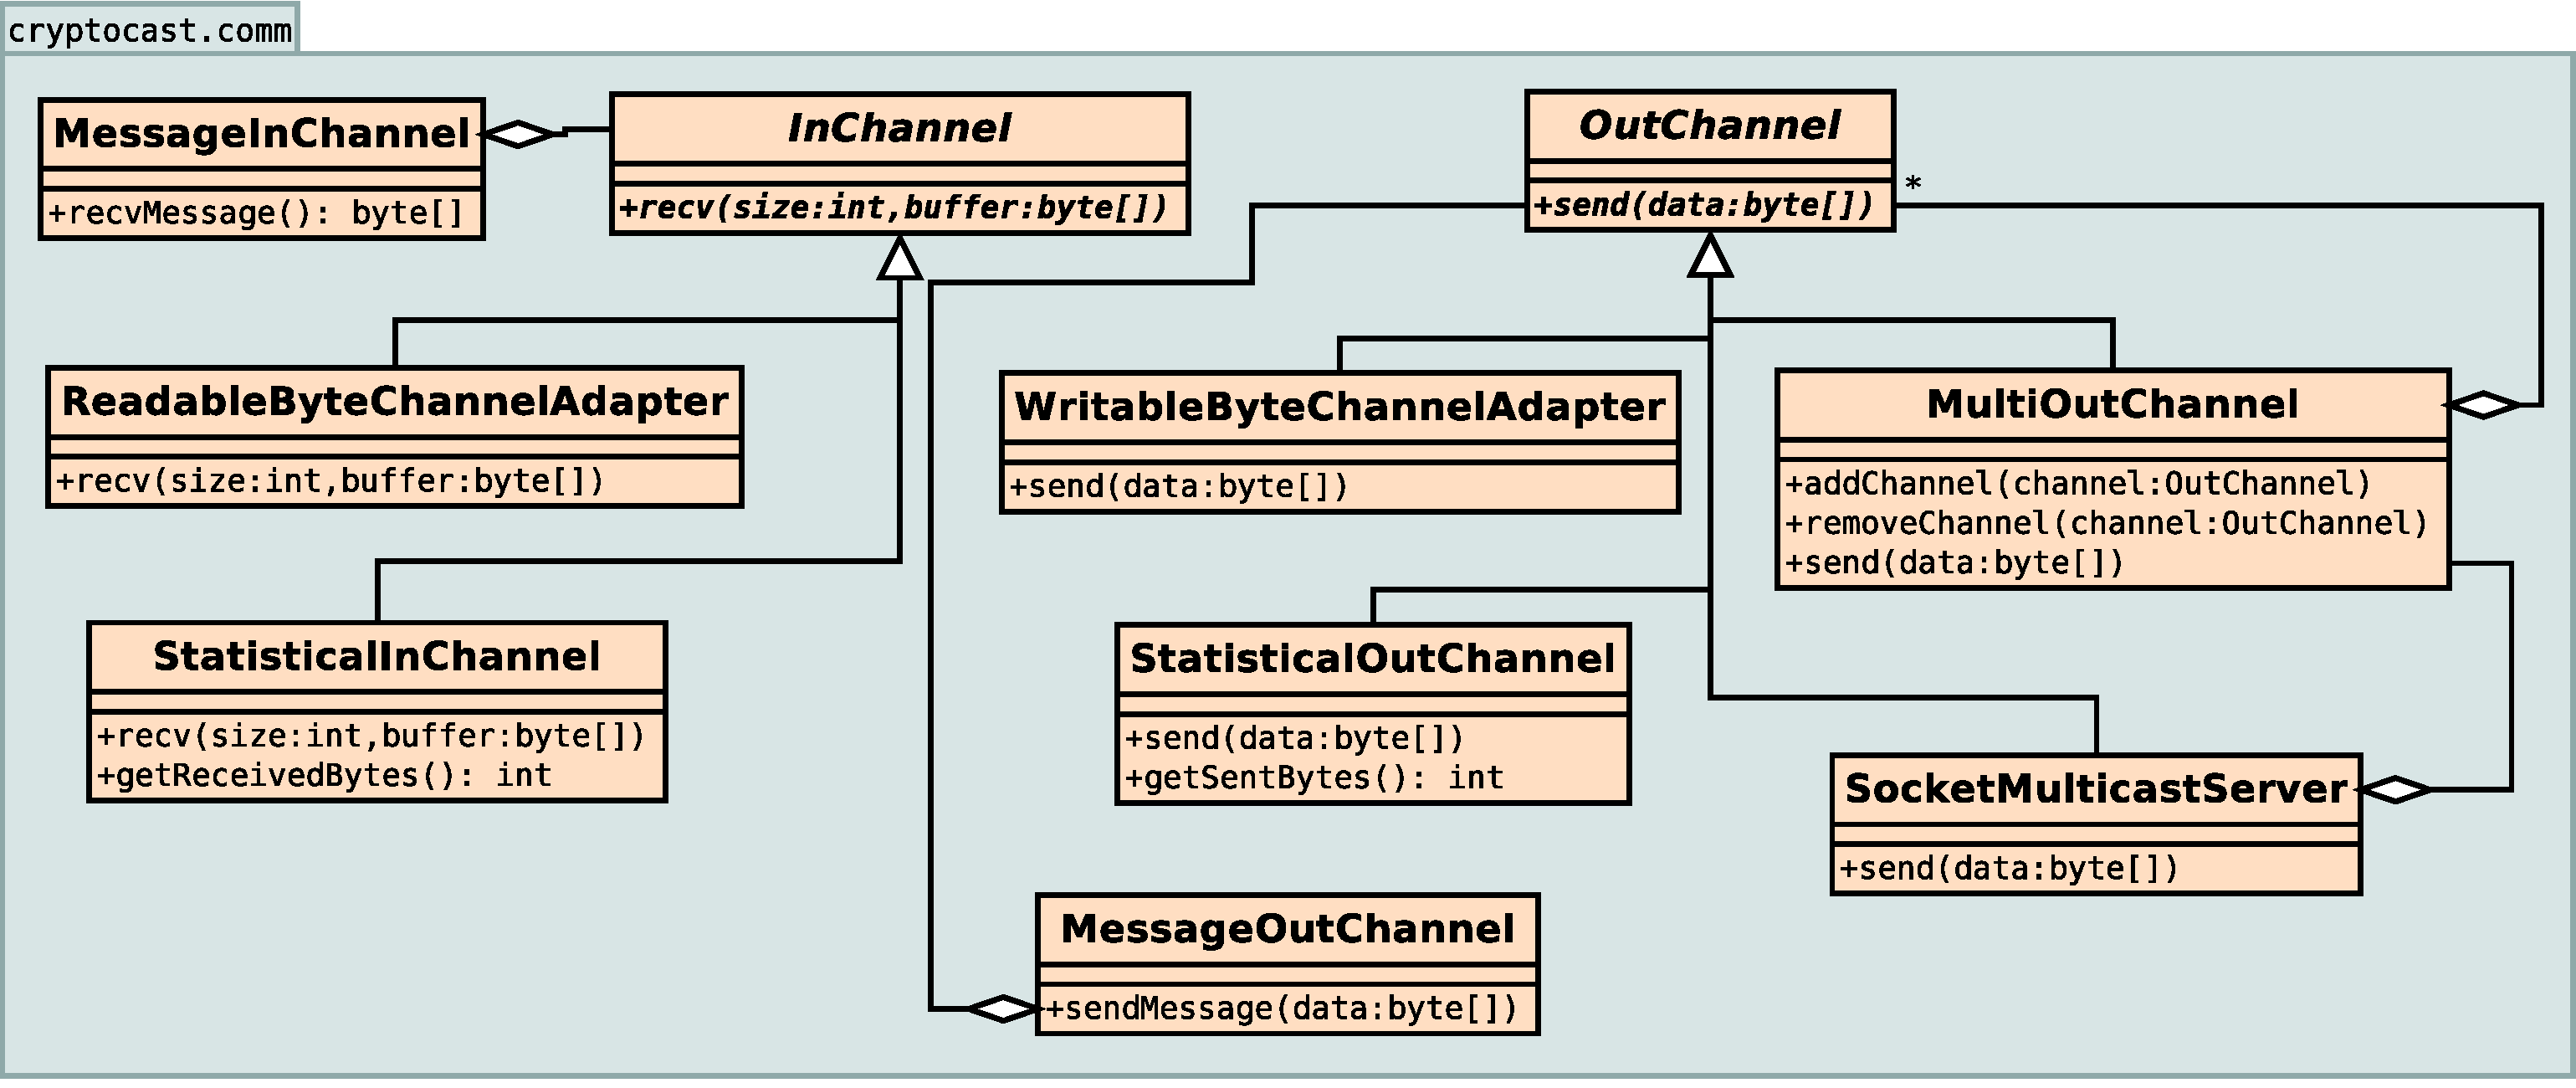
\includegraphics[width=450px]{class_diagrams/cryptocast_comm.pdf}
\end{minipage}

\subsubsection{Class \lstinline|WritableByteChannelAdapter|}
Adapter to use a \lstinline|WritableByteChannel| (for example, a file or socket instance) as
 an \lstinline|OutChannel|. \\
\noindent\begin{minipage}[t]{5cm}
\vspace{0.3em}
\hspace*{2em}
\begin{tikzpicture}
\umlclass[]{WritableByteChannelAdapter}{

}{
+ send(data : byte[])
}
\end{tikzpicture}
\vspace{0.3em}
\end{minipage}



\textbf{\sffamily Superclasses and Interfaces}
\begin{itemize}
\item \lstinline|cryptocast.comm.OutChannel|
\end{itemize}


\textbf{\sffamily Constructors}
\begin{itemize}
\item \lstinline|public| \lstinline|WritableByteChannelAdapter|\lstinline|(WritableByteChannel inner)|\\ \\[-0.6em]
Initializes the adapter
\begin{itemize}
\item \lstinline|inner|: The wrapped instance
\end{itemize}



\end{itemize}


\textbf{\sffamily Methods}
\begin{itemize}
\item \lstinline|public void| \lstinline|send|\lstinline|(byte[] data)|\\ \\[-0.6em]
Sends the given data.
\begin{itemize}
\item \lstinline|data|: the data to send
\end{itemize}



\end{itemize}

\subsubsection{Class \lstinline|StatisticalOutChannel|}
Wrapper around an \lstinline|OutChannel| that counts outgoing bytes. \\
\noindent\begin{minipage}[t]{5cm}
\vspace{0.3em}
\hspace*{2em}
\begin{tikzpicture}
\umlclass[]{StatisticalOutChannel}{

}{
+ send(data : byte[]) \\ + getSentBytes() : int
}
\end{tikzpicture}
\vspace{0.3em}
\end{minipage}



\textbf{\sffamily Superclasses and Interfaces}
\begin{itemize}
\item \lstinline|cryptocast.comm.OutChannel|
\end{itemize}


\textbf{\sffamily Constructors}
\begin{itemize}
\item \lstinline|public| \lstinline|StatisticalOutChannel|\lstinline|(OutChannel inner)|\\ \\[-0.6em]
Initializes the proxy
\begin{itemize}
\item \lstinline|inner|: the wrapped channel
\end{itemize}



\end{itemize}


\textbf{\sffamily Methods}
\begin{itemize}
\item \lstinline|public void| \lstinline|send|\lstinline|(byte[] data)|\\ \\[-0.6em]
Sends the given data.
\begin{itemize}
\item \lstinline|data|: the data to send
\end{itemize}



\item \lstinline|public int| \lstinline|getSentBytes|\lstinline|()|\\ \\[-0.6em]
\emph{Returns:} the number of sent bytes



\end{itemize}

\subsubsection{Class \lstinline|SocketMulticastServer|}
This class implements channel-based communication via TCP. \\
\noindent\begin{minipage}[t]{5cm}
\vspace{0.3em}
\hspace*{2em}
\begin{tikzpicture}
\umlclass[]{SocketMulticastServer}{

}{
+ send(data : byte[])
}
\end{tikzpicture}
\vspace{0.3em}
\end{minipage}



\textbf{\sffamily Superclasses and Interfaces}
\begin{itemize}
\item \lstinline|cryptocast.comm.OutChannel|
\end{itemize}


\textbf{\sffamily Constructors}
\begin{itemize}
\item \lstinline|public| \lstinline|SocketMulticastServer|\lstinline|(ServerSocket socket)|\\ \\[-0.6em]
Creates a multicast server which uses the given socket.
\begin{itemize}
\item \lstinline|socket|: server socket
\end{itemize}



\end{itemize}


\textbf{\sffamily Methods}
\begin{itemize}
\item \lstinline|public void| \lstinline|send|\lstinline|(byte[] data)|\\ \\[-0.6em]
Sends bytes via the channel.
\begin{itemize}
\item \lstinline|data|: the data to send
\end{itemize}



\end{itemize}

\subsubsection{Class \lstinline|MessageInChannel|}
Wraps a byte-based InChannel and allows to use it as a message-based
 channel. \\
\noindent\begin{minipage}[t]{5cm}
\vspace{0.3em}
\hspace*{2em}
\begin{tikzpicture}
\umlclass[]{MessageInChannel}{

}{
+ recvMessage() : byte[]
}
\end{tikzpicture}
\vspace{0.3em}
\end{minipage}




\textbf{\sffamily Constructors}
\begin{itemize}
\item \lstinline|public| \lstinline|MessageInChannel|\lstinline|(InChannel inner)|\\ \\[-0.6em]
Creates a MessageInChannel which wraps the given inner channel.
\begin{itemize}
\item \lstinline|inner|: the wrapped channel
\end{itemize}



\end{itemize}


\textbf{\sffamily Methods}
\begin{itemize}
\item \lstinline|public byte[]| \lstinline|recvMessage|\lstinline|()|\\ \\[-0.6em]
Receives a message via the channel.

\emph{Returns:} the received data

\end{itemize}

\subsubsection{Class \lstinline|MessageOutChannel|}
Wraps a byte-based OutChannel and allows to use it as a message-based
 channel. \\
\noindent\begin{minipage}[t]{5cm}
\vspace{0.3em}
\hspace*{2em}
\begin{tikzpicture}
\umlclass[]{MessageOutChannel}{

}{
+ sendMessage(data : byte[])
}
\end{tikzpicture}
\vspace{0.3em}
\end{minipage}




\textbf{\sffamily Constructors}
\begin{itemize}
\item \lstinline|public| \lstinline|MessageOutChannel|\lstinline|(OutChannel inner)|\\ \\[-0.6em]
Creates a new MessageOutChannel with the given OutChannel as inner channel.
\begin{itemize}
\item \lstinline|inner|: the OutChannel which will be wrapped
\end{itemize}



\end{itemize}


\textbf{\sffamily Methods}
\begin{itemize}
\item \lstinline|public void| \lstinline|sendMessage|\lstinline|(byte[] data)|\\ \\[-0.6em]
Sends the given message via the channel.
\begin{itemize}
\item \lstinline|data|: the data to send
\end{itemize}



\end{itemize}

\subsubsection{Class \lstinline|StatisticalInChannel|}
Wrapper around an \lstinline|InChannel| that counts incoming bytes \\
\noindent\begin{minipage}[t]{5cm}
\vspace{0.3em}
\hspace*{2em}
\begin{tikzpicture}
\umlclass[]{StatisticalInChannel}{

}{
+ recv(size : int, buffer : byte[]) \\ + getReceivedBytes() : int
}
\end{tikzpicture}
\vspace{0.3em}
\end{minipage}



\textbf{\sffamily Superclasses and Interfaces}
\begin{itemize}
\item \lstinline|cryptocast.comm.InChannel|
\end{itemize}


\textbf{\sffamily Constructors}
\begin{itemize}
\item \lstinline|public| \lstinline|StatisticalInChannel|\lstinline|(InChannel inner)|\\ \\[-0.6em]
Initializes the proxy
\begin{itemize}
\item \lstinline|inner|: the wrapped channel
\end{itemize}



\end{itemize}


\textbf{\sffamily Methods}
\begin{itemize}
\item \lstinline|public void| \lstinline|recv|\lstinline|(int size, byte[] buffer)|\\ \\[-0.6em]
Receives data.
\begin{itemize}
\item \lstinline|size|: maximum amount of bytes to read
\item \lstinline|buffer|: the target buffer
\end{itemize}



\item \lstinline|public int| \lstinline|getReceivedBytes|\lstinline|()|\\ \\[-0.6em]
\emph{Returns:} the number of received bytes



\end{itemize}

\subsubsection{Class \lstinline|ReadableByteChannelAdapter|}
Adapter to use a \lstinline|ReadableByteChannel| (for example, a file or socket instance) as an
 \lstinline|InChannel|. \\
\noindent\begin{minipage}[t]{5cm}
\vspace{0.3em}
\hspace*{2em}
\begin{tikzpicture}
\umlclass[]{ReadableByteChannelAdapter}{

}{
+ recv(size : int, buffer : byte[])
}
\end{tikzpicture}
\vspace{0.3em}
\end{minipage}



\textbf{\sffamily Superclasses and Interfaces}
\begin{itemize}
\item \lstinline|cryptocast.comm.InChannel|
\end{itemize}


\textbf{\sffamily Constructors}
\begin{itemize}
\item \lstinline|public| \lstinline|ReadableByteChannelAdapter|\lstinline|(ReadableByteChannel inner)|\\ \\[-0.6em]
Initializes the adapter
\begin{itemize}
\item \lstinline|inner|: The wrapped instance
\end{itemize}



\end{itemize}


\textbf{\sffamily Methods}
\begin{itemize}
\item \lstinline|public void| \lstinline|recv|\lstinline|(int size, byte[] buffer)|\\ \\[-0.6em]
Receives data.
\begin{itemize}
\item \lstinline|size|: maximum amount of bytes to read
\item \lstinline|buffer|: the target buffer
\end{itemize}



\end{itemize}

\subsubsection{Class \lstinline|MultiOutChannel|}
Multiplexes several \lstinline|OutChannel|s so that they can be used as a single
 destination. \\
\noindent\begin{minipage}[t]{5cm}
\vspace{0.3em}
\hspace*{2em}
\begin{tikzpicture}
\umlclass[]{MultiOutChannel}{

}{
+ addChannel(channel : OutChannel) \\ + removeChannel(channel : OutChannel) \\ + send(data : byte[])
}
\end{tikzpicture}
\vspace{0.3em}
\end{minipage}



\textbf{\sffamily Superclasses and Interfaces}
\begin{itemize}
\item \lstinline|cryptocast.comm.OutChannel|
\end{itemize}



\textbf{\sffamily Methods}
\begin{itemize}
\item \lstinline|public void| \lstinline|addChannel|\lstinline|(OutChannel channel)|\\ \\[-0.6em]
Adds the given channel to the list of receivers.
\begin{itemize}
\item \lstinline|channel|: the channel to add
\end{itemize}



\item \lstinline|public void| \lstinline|removeChannel|\lstinline|(OutChannel channel)|\\ \\[-0.6em]
Removes the given channel from the list of receivers.
\begin{itemize}
\item \lstinline|channel|: the channel to remove
\end{itemize}



\item \lstinline|public void| \lstinline|send|\lstinline|(byte[] data)|\\ \\[-0.6em]
Sends the given data.
\begin{itemize}
\item \lstinline|data|: the data to send
\end{itemize}



\end{itemize}

\subsubsection{Interface \lstinline|InChannel|}
A byte-based communication channel from which data can be received. \\
\noindent\begin{minipage}[t]{5cm}
\vspace{0.3em}
\hspace*{2em}
\begin{tikzpicture}
\umlclass[type=abstract]{InChannel}{

}{
\umlvirt{+ recv(size : int, buffer : byte[])}
}
\end{tikzpicture}
\vspace{0.3em}
\end{minipage}





\textbf{\sffamily Methods}
\begin{itemize}
\item \lstinline|public void| \lstinline|recv|\lstinline|(int size, byte[] buffer)|\\ \\[-0.6em]
Receives data.
\begin{itemize}
\item \lstinline|size|: maximum amount of bytes to read
\item \lstinline|buffer|: The target buffer
\end{itemize}



\end{itemize}

\subsubsection{Interface \lstinline|OutChannel|}
A byte-based communication channel where data can be sent to. \\
\noindent\begin{minipage}[t]{5cm}
\vspace{0.3em}
\hspace*{2em}
\begin{tikzpicture}
\umlclass[type=abstract]{OutChannel}{

}{
\umlvirt{+ send(data : byte[])}
}
\end{tikzpicture}
\vspace{0.3em}
\end{minipage}





\textbf{\sffamily Methods}
\begin{itemize}
\item \lstinline|public void| \lstinline|send|\lstinline|(byte[] data)|\\ \\[-0.6em]
Sends the given data.
\begin{itemize}
\item \lstinline|data|: the data to send
\end{itemize}



\end{itemize}



\subsection{Package \lstinline!cryptocast.crypto!}

\subsubsection{Class \lstinline|LagrangeInterpolation<T>|}
Performs a lagrange interpolation of a polynomial \\
\begin{tikzpicture}
\umlclass[]{LagrangeInterpolation<T>}{

}{
+ computeCoefficients() : T[]
}
\end{tikzpicture}



\begin{itemize}
\item \lstinline|<T>|: The type of items of the polynomial's field
\end{itemize}


\textbf{Constructors}
\begin{itemize}
\item \lstinline|public| \lstinline|LagrangeInterpolation|\lstinline|(Polynomial<T> poly)|\\
Initializes the algorithm
\begin{itemize}
\item \lstinline|poly|: The polynomial to interpolate
\end{itemize}



\end{itemize}


\textbf{Methods}
\begin{itemize}
\item \lstinline|public T[]| \lstinline|computeCoefficients|\lstinline|()|\\
Returns: The lagrange coefficients of the associated polynomial



\end{itemize}

\subsubsection{Class \lstinline|IntegersModuloPrime|}
The field $\mathbb{Z}/p\mathbb{Z}$ of integers modulo a prime $p$ \\
\begin{tikzpicture}
\umlclass[]{IntegersModuloPrime}{

}{
+ add() : BigInteger \\ + multiply() : BigInteger \\ + negate() : BigInteger \\ + invert() : BigInteger \\ + zero() : BigInteger \\ + one() : BigInteger \\ + randomElement() : BigInteger
}
\end{tikzpicture}



\textbf{Superclasses and Interfaces}
\begin{itemize}
\item \lstinline|cryptocast.crypto.Field<BigInteger>|
\end{itemize}



\textbf{Constructors}
\begin{itemize}
\item \lstinline|public| \lstinline|IntegersModuloPrime|\lstinline|(BigInteger p)|\\
Initializes the field
\begin{itemize}
\item \lstinline|p|: A prime number
\end{itemize}



\end{itemize}


\textbf{Methods}
\begin{itemize}
\item \lstinline|public BigInteger| \lstinline|add|\lstinline|(BigInteger a, BigInteger b)|




\item \lstinline|public BigInteger| \lstinline|multiply|\lstinline|(BigInteger a, BigInteger b)|




\item \lstinline|public BigInteger| \lstinline|negate|\lstinline|(BigInteger a)|




\item \lstinline|public BigInteger| \lstinline|invert|\lstinline|(BigInteger a)|




\item \lstinline|public BigInteger| \lstinline|zero|\lstinline|()|




\item \lstinline|public BigInteger| \lstinline|one|\lstinline|()|




\item \lstinline|public BigInteger| \lstinline|randomElement|\lstinline|()|




\end{itemize}

\subsubsection{Class \lstinline|Polynomial<T>|}
A polynomial $P$ over a field \\
\begin{tikzpicture}
\umlclass[]{Polynomial<T>}{

}{
+ getField() : Field<T> \\ + evaluate() : T \\ + evaluateMulti() : T[] \\ + getCoefficient() : T \\ + getDegree() : int \\ + createRandomPolynomial() : Polynomial<T>
}
\end{tikzpicture}



\begin{itemize}
\item \lstinline|<T>|: The type of the field's elements
\end{itemize}


\textbf{Constructors}
\begin{itemize}
\item \lstinline|public| \lstinline|Polynomial|\lstinline|(Field<T> field, T[] coefficients)|\\
Initializes a polynomial
\begin{itemize}
\item \lstinline|field|: An instance of the field over which the polynomial is formed
\item \lstinline|coefficients|: The coefficients $c_i$ of the polynomial ($0 \leq i \leq n$).
 The polynomial is defined as $P(x) := \sum_{i=0}^n c_i x^i = c_0 + c_1
 x + ... + c_n x^n$
\end{itemize}



\end{itemize}


\textbf{Methods}
\begin{itemize}
\item \lstinline|public Field<T>| \lstinline|getField|\lstinline|()|\\
Returns: The field associated with this polynomial



\item \lstinline|public T| \lstinline|evaluate|\lstinline|(T x)|\\
Evaluates the polynomial at a single point x.
\begin{itemize}
\item \lstinline|x|: The
\end{itemize}

Returns: P(x)

\item \lstinline|public T[]| \lstinline|evaluateMulti|\lstinline|(T[] xs)|\\
Evaluates the polynomial at multiple points in time complexity $\Theta(n\cdot\log
 n)$ where $n$ is the degree of the polynomial
\begin{itemize}
\item \lstinline|xs|: The points $x_i$ to evaluate
\end{itemize}

Returns: The array a defined by $a_i := P(x_i)$

\item \lstinline|public T| \lstinline|getCoefficient|\lstinline|(int i)|\\
Returns: $c_i$
\begin{itemize}
\item \lstinline|i|: The index of the coefficient to get ($0 \leq i \leq n$), where
          $n$ is the degree of the polynomial
\end{itemize}



\item \lstinline|public int| \lstinline|getDegree|\lstinline|()|\\
Returns: The degree of the polynomial



\item \lstinline|public static Polynomial<T>| \lstinline|createRandomPolynomial|\lstinline|(Field<T> field, int degree)|\\
Generates a random polynomial over the field
\begin{itemize}
\item \lstinline|field|: An instance of the field over which the polynomial is formed
\item \lstinline|degree|: The degree of the generated polynomial
\end{itemize}

Returns: The generated polynomial

\end{itemize}

\subsubsection{Class \lstinline|Field<T>|}
Represents a field over values of type T \\
\begin{tikzpicture}
\umlclass[type=abstract]{Field<T>}{

}{
+ add() : T \\ + multiply() : T \\ + negate() : T \\ + invert() : T \\ + zero() : T \\ + one() : T \\ + randomElement() : T \\ + subtract() : T \\ + divide() : T \\ + pow() : T
}
\end{tikzpicture}



\begin{itemize}
\item \lstinline|<T>|: The values we work on
\end{itemize}


\textbf{Constructors}
\begin{itemize}
\item \lstinline|public| \lstinline|Field|\lstinline|()|




\end{itemize}


\textbf{Methods}
\begin{itemize}
\item \lstinline|public abstract T| \lstinline|add|\lstinline|(T a, T b)|\\
Adds two elements of the field
\begin{itemize}
\item \lstinline|a|: first element
\item \lstinline|b|: second element
\end{itemize}

Returns: The value $a + b$

\item \lstinline|public abstract T| \lstinline|multiply|\lstinline|(T a, T b)|\\
Multiplies two elements of the field
\begin{itemize}
\item \lstinline|a|: first element
\item \lstinline|b|: second element
\end{itemize}

Returns: The value $a \cdot b$

\item \lstinline|public abstract T| \lstinline|negate|\lstinline|(T a)|\\
Returns: The additive inverse $-a$ of $a$
\begin{itemize}
\item \lstinline|a|: An element of the field
\end{itemize}



\item \lstinline|public abstract T| \lstinline|invert|\lstinline|(T a)|\\
Returns: The multiplicative inverse $a^{-1}$ of $a$
\begin{itemize}
\item \lstinline|a|: An element of the field
\end{itemize}



\item \lstinline|public abstract T| \lstinline|zero|\lstinline|()|\\
Returns: The zero element of the field



\item \lstinline|public abstract T| \lstinline|one|\lstinline|()|\\
Returns: The one element of the field



\item \lstinline|public abstract T| \lstinline|randomElement|\lstinline|()|\\
Returns: A random element of the field



\item \lstinline|public T| \lstinline|subtract|\lstinline|(T a, T b)|\\
Subtracts two elements of the field
\begin{itemize}
\item \lstinline|a|: first element
\item \lstinline|b|: second element
\end{itemize}

Returns: The value $a - b$

\item \lstinline|public T| \lstinline|divide|\lstinline|(T a, T b)|\\
Divides two elements of the field
\begin{itemize}
\item \lstinline|a|: first element
\item \lstinline|b|: second element
\end{itemize}

Returns: The value $\frac{a}{b}$

\item \lstinline|public T| \lstinline|pow|\lstinline|(T a, int e)|\\
Raises an element of the field to an integer power
\begin{itemize}
\item \lstinline|a|: The element of the field
\item \lstinline|e|: The exponent
\end{itemize}

Returns: The value $a^e$

\end{itemize}

\subsubsection{Class \lstinline|BroadcastEncryptionServer<ID>|}
The server side of a broadcast encryption scheme. \\
\begin{tikzpicture}
\umlclass[]{BroadcastEncryptionServer<ID>}{

}{
+ run() : void \\ + send() : void \\ + revoke() : void
}
\end{tikzpicture}



\textbf{Superclasses and Interfaces}
\begin{itemize}
\item \lstinline|cryptocast.comm.OutChannel|
\item \lstinline|java.lang.Runnable|
\end{itemize}

\begin{itemize}
\item \lstinline|<ID>|: The type of the identities
\end{itemize}


\textbf{Constructors}
\begin{itemize}
\item \lstinline|public| \lstinline|BroadcastEncryptionServer|\lstinline|(MessageOutChannel inner, BroadcastSchemeUserManager<ID> context, Encryptor<BigInteger> enc)|\\
Initializes a broadcast encryption server.
\begin{itemize}
\item \lstinline|inner|: The message-based communication channel to send outgoing data to
\item \lstinline|context|: The user management context
\item \lstinline|enc|: The encryption context
\end{itemize}



\end{itemize}


\textbf{Methods}
\begin{itemize}
\item \lstinline|public void| \lstinline|run|\lstinline|()|\\
Run the worker that handles periodic group key broadcasts and sends
 queued data packages.



\item \lstinline|public void| \lstinline|send|\lstinline|(byte[] data)|\\
Send plaintext data to the channel. It will be encryted and broadcasted
 on the fly.
\begin{itemize}
\item \lstinline|data|: The data to send
\end{itemize}



\item \lstinline|public void| \lstinline|revoke|\lstinline|(ID id)|\\
Revoke a user.
\begin{itemize}
\item \lstinline|id|: The identity of the user
\end{itemize}



\end{itemize}

\subsubsection{Class \lstinline|BroadcastEncryptionClient|}
The client side of a broadcast encryption scheme. \\
\begin{tikzpicture}
\umlclass[]{BroadcastEncryptionClient}{

}{
+ recv() : void
}
\end{tikzpicture}



\textbf{Superclasses and Interfaces}
\begin{itemize}
\item \lstinline|cryptocast.comm.InChannel|
\end{itemize}



\textbf{Constructors}
\begin{itemize}
\item \lstinline|public| \lstinline|BroadcastEncryptionClient|\lstinline|(MessageInChannel inner, Decryptor<BigInteger> dec)|\\
Initializes a broadcast encryption client.
\begin{itemize}
\item \lstinline|inner|: The message-based underlying communication channel.
\item \lstinline|dec|: The decryption context
\end{itemize}



\end{itemize}


\textbf{Methods}
\begin{itemize}
\item \lstinline|public void| \lstinline|recv|\lstinline|(int size, byte[] buffer)|\\
Receive data from the channel. It is decrypted on the fly.
\begin{itemize}
\item \lstinline|size|: amount of bytes to receive
\item \lstinline|buffer|: the target buffer
\end{itemize}



\end{itemize}

\subsubsection{Interface \lstinline|Decryptor<S>|}
A strategy to decrypt a single secret \\
\begin{tikzpicture}
\umlclass[type=abstract]{Decryptor<S>}{

}{
+ decrypt() : S
}
\end{tikzpicture}



\begin{itemize}
\item \lstinline|<S>|: the type of the secret
\end{itemize}



\textbf{Methods}
\begin{itemize}
\item \lstinline|public S| \lstinline|decrypt|\lstinline|(byte[] cipher)|\\
Decrypts a secret.
\begin{itemize}
\item \lstinline|cipher|: The encrypted secret
\end{itemize}

Returns: The decrypted secret

\end{itemize}

\subsubsection{Interface \lstinline|BroadcastSchemeUserManager<ID>|}
Manages a set of user identites \\
\begin{tikzpicture}
\umlclass[type=abstract]{BroadcastSchemeUserManager<ID>}{

}{
+ getIdentity() : ID \\ + revoke() : void \\ + isRevoked() : boolean
}
\end{tikzpicture}



\begin{itemize}
\item \lstinline|<ID>|: The type of the identities
\end{itemize}



\textbf{Methods}
\begin{itemize}
\item \lstinline|public ID| \lstinline|getIdentity|\lstinline|(int i)|\\
Returns: The identity with the given index
\begin{itemize}
\item \lstinline|i|: An index
\end{itemize}



\item \lstinline|public void| \lstinline|revoke|\lstinline|(ID id)|\\
Revokes a user
\begin{itemize}
\item \lstinline|id|: The identity of the user
\end{itemize}



\item \lstinline|public boolean| \lstinline|isRevoked|\lstinline|(ID id)|\\
Returns: whether the user is revoked
\begin{itemize}
\item \lstinline|id|: The identity of the user
\end{itemize}



\end{itemize}

\subsubsection{Interface \lstinline|Encryptor<S>|}
A strategy to encrypt a single secret \\
\begin{tikzpicture}
\umlclass[type=abstract]{Encryptor<S>}{

}{
+ encrypt() : byte[]
}
\end{tikzpicture}



\begin{itemize}
\item \lstinline|<S>|: the type of the secret
\end{itemize}



\textbf{Methods}
\begin{itemize}
\item \lstinline|public byte[]| \lstinline|encrypt|\lstinline|(S secret)|\\
Encrypts a secret
\begin{itemize}
\item \lstinline|secret|: the secret
\end{itemize}

Returns: The cipher text

\end{itemize}

\subsubsection{Interface \lstinline|BroadcastSchemeKeyManager<ID>|}
Manages the private keys of a set of users. \\
\begin{tikzpicture}
\umlclass[type=abstract]{BroadcastSchemeKeyManager<ID>}{

}{
+ getPersonalKey() : PrivateKey
}
\end{tikzpicture}



\begin{itemize}
\item \lstinline|<ID>|: The type of the user identities
\end{itemize}



\textbf{Methods}
\begin{itemize}
\item \lstinline|public PrivateKey| \lstinline|getPersonalKey|\lstinline|(ID id)|\\
Returns: The private key of the user
\begin{itemize}
\item \lstinline|id|: The identity to look up
\end{itemize}



\end{itemize}

\subsubsection{Interface \lstinline|ShareCombinator<S, T>|}
Implements a strategy to restore a secret from a number of shares. \\
\begin{tikzpicture}
\umlclass[type=abstract]{ShareCombinator<S, T>}{

}{
+ restore() : <any>
}
\end{tikzpicture}



\begin{itemize}
\item \lstinline|<S>|: The type of the secret
\item \lstinline|<T>|: The type of the shares
\end{itemize}



\textbf{Methods}
\begin{itemize}
\item \lstinline|public <any>| \lstinline|restore|\lstinline|(Collection<T> shares)|\\
Restores a secret from several shares.

Returns: The reconstructed secret or absent if the information represented
 by the given shares is insufficient to restore it.

\end{itemize}



\subsection{Package \lstinline!cryptocast.crypto.naorpinkas!}

\subsubsection{Class \lstinline|NaorPinkasClient|}
A client in the Naor-Pinkas broadcast encryption scheme. \\
\noindent\begin{minipage}[t]{5cm}
\vspace{0.3em}
\hspace*{2em}
\begin{tikzpicture}
\umlclass[]{NaorPinkasClient}{

}{
+ decrypt(cipher : byte[]) : BigInteger
}
\end{tikzpicture}
\vspace{0.3em}
\end{minipage}



\textbf{\sffamily Superclasses and Interfaces}
\begin{itemize}
\item \lstinline|cryptocast.crypto.Decryptor<BigInteger>|
\end{itemize}


\textbf{\sffamily Constructors}
\begin{itemize}
\item \lstinline|public| \lstinline|NaorPinkasClient|\lstinline|(NaorPinkasPersonalKey key)|\\ \\[-0.6em]
Initializes a Naor-Pinkas broadcast client
\begin{itemize}
\item \lstinline|key|: The personal key used to reconstruct a secret from the stream
\end{itemize}



\end{itemize}


\textbf{\sffamily Methods}
\begin{itemize}
\item \lstinline|public BigInteger| \lstinline|decrypt|\lstinline|(byte[] cipher)|\\ \\[-0.6em]
Decrypts a secret.
\begin{itemize}
\item \lstinline|cipher|: The encrypted secret
\end{itemize}

\emph{Returns:} The decrypted secret

\end{itemize}

\subsubsection{Class \lstinline|NaorPinkasServer|}
A server in the Naor-Pinkas broadcast encryption scheme. This server is special in that it knows
 the entire polynomial and therefore all the private keys of its users. This makes the implementation
 of the interpolation algorithm a bit more efficient. \\
\noindent\begin{minipage}[t]{5cm}
\vspace{0.3em}
\hspace*{2em}
\begin{tikzpicture}
\umlclass[]{NaorPinkasServer}{

}{
+ encrypt(secret : BigInteger) : byte[] \\ + getIdentity(i : int) : NaorPinkasIdentity \\ + revoke(x : NaorPinkasIdentity) \\ + isRevoked(id : NaorPinkasIdentity) : boolean \\ + getPersonalKey(id : NaorPinkasIdentity) : NaorPinkasPersonalKey
}
\end{tikzpicture}
\vspace{0.3em}
\end{minipage}



\textbf{\sffamily Superclasses and Interfaces}
\begin{itemize}
\item \lstinline|cryptocast.crypto.BroadcastSchemeKeyManager<NaorPinkasIdentity>|
\item \lstinline|cryptocast.crypto.BroadcastSchemeUserManager<NaorPinkasIdentity>|
\item \lstinline|cryptocast.crypto.Encryptor<BigInteger>|
\item \lstinline|java.io.Serializable|
\end{itemize}



\textbf{\sffamily Methods}
\begin{itemize}
\item \lstinline|public byte[]| \lstinline|encrypt|\lstinline|(BigInteger secret)|\\ \\[-0.6em]
Encrypts a secret
\begin{itemize}
\item \lstinline|secret|: the secret
\end{itemize}

\emph{Returns:} The cipher text

\item \lstinline|public NaorPinkasIdentity| \lstinline|getIdentity|\lstinline|(int i)|\\ \\[-0.6em]
\emph{Returns:} The identity with the given index
\begin{itemize}
\item \lstinline|i|: An index
\end{itemize}



\item \lstinline|public void| \lstinline|revoke|\lstinline|(NaorPinkasIdentity x)|\\ \\[-0.6em]
Revokes a user



\item \lstinline|public boolean| \lstinline|isRevoked|\lstinline|(NaorPinkasIdentity id)|\\ \\[-0.6em]
\emph{Returns:} whether the user is revoked
\begin{itemize}
\item \lstinline|id|: The identity of the user
\end{itemize}



\item \lstinline|public NaorPinkasPersonalKey| \lstinline|getPersonalKey|\lstinline|(NaorPinkasIdentity id)|\\ \\[-0.6em]
\emph{Returns:} The private key of the user
\begin{itemize}
\item \lstinline|id|: The identity to look up
\end{itemize}



\end{itemize}

\subsubsection{Class \lstinline|NaorPinkasPersonalKey|}
A user's personal key in the Naor-Pinkas broadcast encryption scheme. \\
\noindent\begin{minipage}[t]{5cm}
\vspace{0.3em}
\hspace*{2em}
\begin{tikzpicture}
\umlclass[]{NaorPinkasPersonalKey}{

}{
+ getAlgorithm() : String \\ + getEncoded() : byte[] \\ + getFormat() : String
}
\end{tikzpicture}
\vspace{0.3em}
\end{minipage}



\textbf{\sffamily Superclasses and Interfaces}
\begin{itemize}
\item \lstinline|java.security.PrivateKey|
\end{itemize}



\textbf{\sffamily Methods}
\begin{itemize}
\item \lstinline|public String| \lstinline|getAlgorithm|\lstinline|()| \\[-0.6em]




\item \lstinline|public byte[]| \lstinline|getEncoded|\lstinline|()| \\[-0.6em]




\item \lstinline|public String| \lstinline|getFormat|\lstinline|()| \\[-0.6em]




\end{itemize}

\subsubsection{Class \lstinline|NaorPinkasShareCombinator|}
Allows to restore a number from a sufficient number of Naor-Pinkas shares \\
\noindent\begin{minipage}[t]{5cm}
\vspace{0.3em}
\hspace*{2em}
\begin{tikzpicture}
\umlclass[]{NaorPinkasShareCombinator}{

}{
+ restore(shares : Collection<NaorPinkasShare>) : Optional<BigInteger>
}
\end{tikzpicture}
\vspace{0.3em}
\end{minipage}



\textbf{\sffamily Superclasses and Interfaces}
\begin{itemize}
\item \lstinline|cryptocast.crypto.ShareCombinator<BigInteger, NaorPinkasShare>|
\end{itemize}



\textbf{\sffamily Methods}
\begin{itemize}
\item \lstinline|public Optional<BigInteger>| \lstinline|restore|\lstinline|(Collection<NaorPinkasShare> shares)|\\ \\[-0.6em]
Restores a secret from several Naor-Pinkas shares.

\emph{Returns:} The reconstructed secret or absent if the information represented
 by the given shares is insufficient to restore it.

\end{itemize}

\subsubsection{Class \lstinline|NaorPinkasShare|}
A share in the Naor-Pinkas broadcast encryption scheme. It consists of a tuple
 $(r, I, g^{r P(I)})$. $t + 1$ distinct shares of this form are sufficient to restore the
 value $g^{r P(0)}$, where $t$ is the degree of the polynomial $P$. \\
\noindent\begin{minipage}[t]{5cm}
\vspace{0.3em}
\hspace*{2em}
\begin{tikzpicture}
\umlclass[]{NaorPinkasShare}{

}{

}
\end{tikzpicture}
\vspace{0.3em}
\end{minipage}





\subsubsection{Class \lstinline|NaorPinkasIdentity|}
An identity in the Naor-Pinkas broadcast encryption scheme \\
\noindent\begin{minipage}[t]{5cm}
\vspace{0.3em}
\hspace*{2em}
\begin{tikzpicture}
\umlclass[]{NaorPinkasIdentity}{

}{
-- getId() : BigInteger
}
\end{tikzpicture}
\vspace{0.3em}
\end{minipage}




\textbf{\sffamily Constructors}
\begin{itemize}
\item \lstinline|private| \lstinline|NaorPinkasIdentity|\lstinline|(BigInteger id)| \\[-0.6em]




\end{itemize}


\textbf{\sffamily Methods}
\begin{itemize}
\item \lstinline|private BigInteger| \lstinline|getId|\lstinline|()| \\[-0.6em]




\end{itemize}



\subsection{Package \lstinline!cryptocast.util!}
Utility classes that are not specific to CryptoCast and don't fit any of the other packages.

\noindent\begin{minipage}[t]{5cm}
\vspace{0.3em}
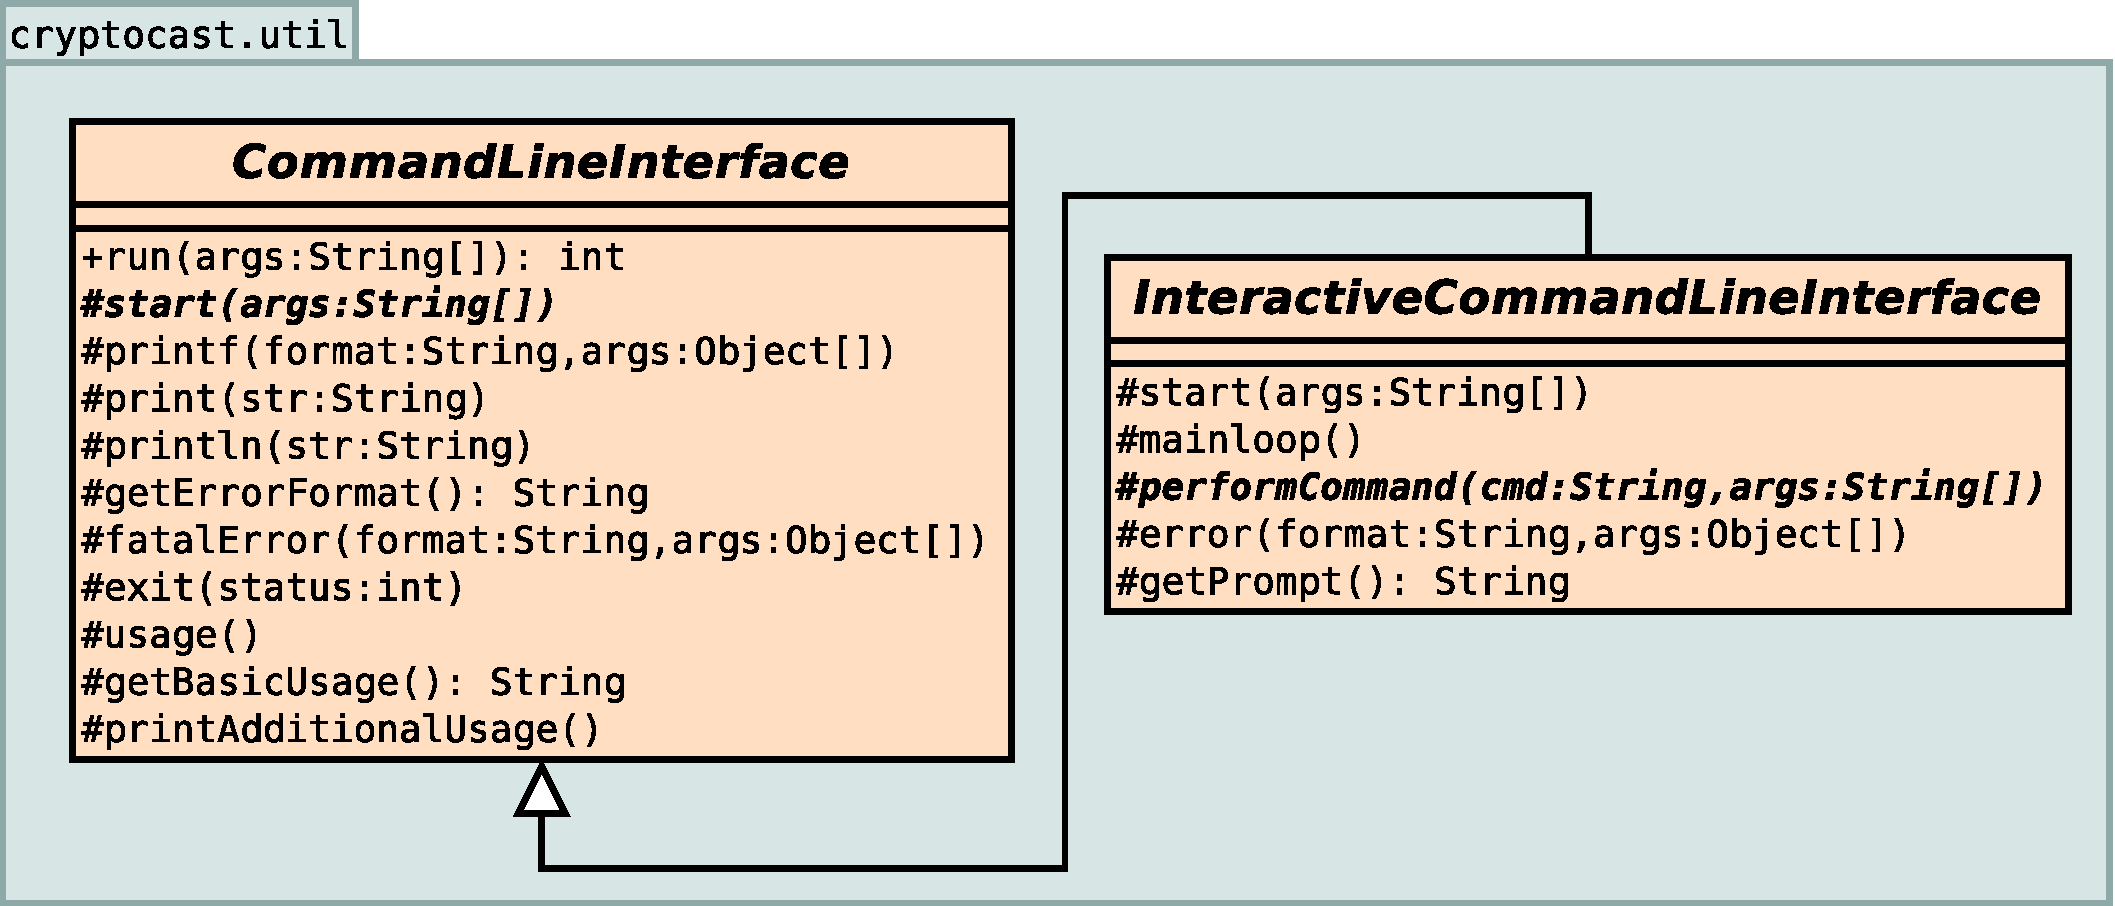
\includegraphics[width=300px]{class_diagrams/cryptocast_util.pdf}
\end{minipage}

\subsubsection{Class \lstinline|CommandLineInterface|}
A simple framework for command line programs. \\
\noindent\begin{minipage}[t]{5cm}
\vspace{0.3em}
\hspace*{2em}
\begin{tikzpicture}
\umlclass[type=abstract]{CommandLineInterface}{

}{
+ run(args : String[]) : int \\ \umlvirt{\# start(args : String[])} \\ \# printf(format : String, args : Object[]...) \\ \# print(str : String) \\ \# println(str : String) \\ \# getErrorFormat() : String \\ \# fatalError(format : String, args : Object[]...) \\ \# exit(status : int) \\ \# usage() \\ \# getBasicUsage() : String \\ \# printAdditionalUsage()
}
\end{tikzpicture}
\vspace{0.3em}
\end{minipage}




\textbf{\sffamily Constructors}
\begin{itemize}
\item \lstinline|public| \lstinline|CommandLineInterface|\lstinline|(InputStream in, PrintStream out, PrintStream err)|\\ \\[-0.6em]
Initializes a new CLI instance.
\begin{itemize}
\item \lstinline|in|: The stream for program input
\item \lstinline|out|: The stream for program output
\item \lstinline|err|: The stream for error output
\end{itemize}



\end{itemize}


\textbf{\sffamily Methods}
\begin{itemize}
\item \lstinline|public int| \lstinline|run|\lstinline|(String[] args)|\\ \\[-0.6em]
Runs the application.
\begin{itemize}
\item \lstinline|args|: The command line arguments
\end{itemize}

\emph{Returns:} The exit code

\item \lstinline|protected abstract void| \lstinline|start|\lstinline|(String[] args)|\\ \\[-0.6em]
The main program logic (must be overridden by subclasses)
\begin{itemize}
\item \lstinline|args|: The command line arguments
\end{itemize}



\item \lstinline|protected void| \lstinline|printf|\lstinline|(String format, Object[] args...)|\\ \\[-0.6em]
Prints a string to the output stream.
\begin{itemize}
\item \lstinline|format|: The string to print (printf format string).
\item \lstinline|args|: The printf arguments
\end{itemize}



\item \lstinline|protected void| \lstinline|print|\lstinline|(String str)|\\ \\[-0.6em]
Prints a string to the output stream.
\begin{itemize}
\item \lstinline|str|: The string to print.
\end{itemize}



\item \lstinline|protected void| \lstinline|println|\lstinline|(String str)|\\ \\[-0.6em]
Prints a string to the output stream after appending a newline.
\begin{itemize}
\item \lstinline|str|: The string to print.
\end{itemize}



\item \lstinline|protected String| \lstinline|getErrorFormat|\lstinline|()|\\ \\[-0.6em]
\emph{Returns:} The string format to use for writing error messages to the
 screen.



\item \lstinline|protected void| \lstinline|fatalError|\lstinline|(String format, Object[] args...)|\\ \\[-0.6em]
Prints an error and exits.
\begin{itemize}
\item \lstinline|format|: The error message (printf format string)
\item \lstinline|args|: The printf arguments
\end{itemize}



\item \lstinline|protected void| \lstinline|exit|\lstinline|(int status)|\\ \\[-0.6em]
Exits the application.
\begin{itemize}
\item \lstinline|status|: The exit code
\end{itemize}



\item \lstinline|protected void| \lstinline|usage|\lstinline|()|\\ \\[-0.6em]
Prints usage information.



\item \lstinline|protected String| \lstinline|getBasicUsage|\lstinline|()|\\ \\[-0.6em]
\emph{Returns:} basic usage information for the program (should be overridden).



\item \lstinline|protected void| \lstinline|printAdditionalUsage|\lstinline|()|\\ \\[-0.6em]
Prints additional usage information (may be overridden).



\end{itemize}

\subsubsection{Class \lstinline|CommandLineInterface.Exit|}
Signals the exit of the application. \\
\noindent\begin{minipage}[t]{5cm}
\vspace{0.3em}
\hspace*{2em}
\begin{tikzpicture}
\umlclass[]{CommandLineInterface.Exit}{

}{
+ getStatus() : int
}
\end{tikzpicture}
\vspace{0.3em}
\end{minipage}



\textbf{\sffamily Superclasses and Interfaces}
\begin{itemize}
\item \lstinline|java.lang.Throwable|
\end{itemize}


\textbf{\sffamily Constructors}
\begin{itemize}
\item \lstinline|public| \lstinline|CommandLineInterface.Exit|\lstinline|(int status)|\\ \\[-0.6em]
Initializes a new Exit instance.
\begin{itemize}
\item \lstinline|status|: The exit code
\end{itemize}



\end{itemize}


\textbf{\sffamily Methods}
\begin{itemize}
\item \lstinline|public int| \lstinline|getStatus|\lstinline|()|\\ \\[-0.6em]
\emph{Returns:} The exit code



\end{itemize}

\subsubsection{Class \lstinline|InteractiveCommandLineInterface|}
A framework class to implement interactive command-line interfaces. The class implements
 a read-parse-execute main loop and provides hooks for subclasses to implement the missing
 functionality. \\
\noindent\begin{minipage}[t]{5cm}
\vspace{0.3em}
\hspace*{2em}
\begin{tikzpicture}
\umlclass[type=abstract]{InteractiveCommandLineInterface}{

}{
\# start(args : String[]) \\ \# mainloop() \\ \umlvirt{\# performCommand(cmd : String, args : String[])} \\ \# error(format : String, args : Object[]...) \\ \# getPrompt() : String
}
\end{tikzpicture}
\vspace{0.3em}
\end{minipage}



\textbf{\sffamily Superclasses and Interfaces}
\begin{itemize}
\item \lstinline|cryptocast.util.CommandLineInterface|
\end{itemize}


\textbf{\sffamily Constructors}
\begin{itemize}
\item \lstinline|public| \lstinline|InteractiveCommandLineInterface|\lstinline|(InputStream in, PrintStream out, PrintStream err)|\\ \\[-0.6em]
Initializes a new interactive CLI instance.
\begin{itemize}
\item \lstinline|in|: The stream for program input
\item \lstinline|out|: The stream for program output
\item \lstinline|err|: The stream for error output
\end{itemize}



\end{itemize}


\textbf{\sffamily Methods}
\begin{itemize}
\item \lstinline|protected void| \lstinline|start|\lstinline|(String[] args)|\\ \\[-0.6em]
The main program logic. This method just starts the main loop.
\begin{itemize}
\item \lstinline|args|: The command line arguments (ignored by default)
\end{itemize}



\item \lstinline|protected void| \lstinline|mainloop|\lstinline|()|\\ \\[-0.6em]
Starts the interactive Prompt-Read-Evaluate main loop.



\item \lstinline|protected abstract void| \lstinline|performCommand|\lstinline|(String cmd, String[] args)|\\ \\[-0.6em]
Executes the given command with the given arguments. Must be implemented by subclasses.
\begin{itemize}
\item \lstinline|cmd|: The command name
\item \lstinline|args|: The command arguments
\end{itemize}



\item \lstinline|protected void| \lstinline|error|\lstinline|(String format, Object[] args...)|\\ \\[-0.6em]
Helper function to trigger an error withing a command's execution and break out to
 the main loop.
\begin{itemize}
\item \lstinline|format|: The format string
\item \lstinline|args|: The format string arguments
\end{itemize}



\item \lstinline|protected String| \lstinline|getPrompt|\lstinline|()|\\ \\[-0.6em]
\emph{Returns:} The input prompt



\end{itemize}

\subsubsection{Class \lstinline|InteractiveCommandLineInterface.CommandError|}
An error within one of the commands. Will be caught by the main loop. \\
\noindent\begin{minipage}[t]{5cm}
\vspace{0.3em}
\hspace*{2em}
\begin{tikzpicture}
\umlclass[]{InteractiveCommandLineInterface.CommandError}{

}{
+ getMessage() : String
}
\end{tikzpicture}
\vspace{0.3em}
\end{minipage}



\textbf{\sffamily Superclasses and Interfaces}
\begin{itemize}
\item \lstinline|java.lang.Throwable|
\end{itemize}


\textbf{\sffamily Constructors}
\begin{itemize}
\item \lstinline|public| \lstinline|InteractiveCommandLineInterface.CommandError|\lstinline|(String msg)|\\ \\[-0.6em]
Initializes the error.
\begin{itemize}
\item \lstinline|msg|: The error message
\end{itemize}



\end{itemize}


\textbf{\sffamily Methods}
\begin{itemize}
\item \lstinline|public String| \lstinline|getMessage|\lstinline|()|\\ \\[-0.6em]
\emph{Returns:} The associated error message.



\end{itemize}



\subsection{Package \lstinline!cryptocast.server!}

\subsubsection{Class \lstinline|Controller<ID>|}
Deals with user-interactions and therefore changes data in Model if necessary. \\
\begin{tikzpicture}
\umlclass[]{Controller<ID>}{

}{
+ init() \\ + keyGen(amtRevocable : int, amtPrivateKeys : int, keyDir : File) \\ + addUser(name : String) \\ + revokeUser(name : String) \\ + authorizeUser(name : String) \\ + stream(data : InputStream) \\ + showStatistics() \\ + showUsers() \\ + showInfo()
}
\end{tikzpicture}



\begin{itemize}
\item \lstinline|<ID>|: The type of the user identities
\end{itemize}


\textbf{Constructors}
\begin{itemize}
\item \lstinline|public| \lstinline|Controller|\lstinline|(ServerData<ID> data, Shell<ID> shell)|\\
Initializes a new controller with the given arguments.
\begin{itemize}
\item \lstinline|data|: The data administrated by this controller.
\item \lstinline|shell|: The operator interface from which this controller gets its input.
\end{itemize}



\end{itemize}


\textbf{Methods}
\begin{itemize}
\item \lstinline|public void| \lstinline|init|\lstinline|()|\\
Initializes the server on start by loading data from a file.



\item \lstinline|public void| \lstinline|keyGen|\lstinline|(int amtRevocable, int amtPrivateKeys, File keyDir)|\\
Tries to start a new group to which data can be sent by generating private keys.
\begin{itemize}
\item \lstinline|amtRevocable|: The amount of user which can be revoked.
\item \lstinline|amtPrivateKeys|: The amount of private keys which are produced.
\item \lstinline|keyDir|: The directory to save the keyfiles in.
\end{itemize}



\item \lstinline|public void| \lstinline|addUser|\lstinline|(String name)|\\
Adds a new user and assigns a private key to that user.
\begin{itemize}
\item \lstinline|name|: The name of the user who is added.
\end{itemize}



\item \lstinline|public void| \lstinline|revokeUser|\lstinline|(String name)|\\
Bans a user from the stream by adding it to the list of revoked users.
\begin{itemize}
\item \lstinline|name|: The name of the user that is revoked.
\end{itemize}



\item \lstinline|public void| \lstinline|authorizeUser|\lstinline|(String name)|\\
Authorizes a user to watch the stream by removing it from the list of revoked users.
\begin{itemize}
\item \lstinline|name|: The name of the user who is unbanned.
\end{itemize}



\item \lstinline|public void| \lstinline|stream|\lstinline|(InputStream data)|\\
Starts the data stream
\begin{itemize}
\item \lstinline|data|: The file from which the data is read
\end{itemize}



\item \lstinline|public void| \lstinline|showStatistics|\lstinline|()|\\
Prints information about traffic



\item \lstinline|public void| \lstinline|showUsers|\lstinline|()|\\
Prints users and the keys assigned to them.



\item \lstinline|public void| \lstinline|showInfo|\lstinline|()|\\
Prints information about the data which is currently sent.



\end{itemize}

\subsubsection{Class \lstinline|User<ID>|}
Represents a user in our application. \\
\begin{tikzpicture}
\umlclass[]{User<ID>}{

}{
+ getName() : String \\ + getIdentity() : ID
}
\end{tikzpicture}



\begin{itemize}
\item \lstinline|<ID>|: The type of the user identities
\end{itemize}


\textbf{Constructors}
\begin{itemize}
\item \lstinline|public| \lstinline|User|\lstinline|(String name, ID id)|\\
Creates a User with the given attributes.
\begin{itemize}
\item \lstinline|name|: The name of this user.
\item \lstinline|id|: The ID of this user.
\end{itemize}



\end{itemize}


\textbf{Methods}
\begin{itemize}
\item \lstinline|public String| \lstinline|getName|\lstinline|()|\\
Returns: the name of this user.



\item \lstinline|public ID| \lstinline|getIdentity|\lstinline|()|\\
Returns: the id of this user.



\end{itemize}

\subsubsection{Class \lstinline|Shell<ID>|}
Gets the arguments from the command line and deals with illegal input. \\
\begin{tikzpicture}
\umlclass[]{Shell<ID>}{

}{
\# performCommand(cmd : String, args : String[]) \\ -- help()
}
\end{tikzpicture}



\textbf{Superclasses and Interfaces}
\begin{itemize}
\item \lstinline|cryptocast.util.InteractiveCommandLineInterface|
\end{itemize}

\begin{itemize}
\item \lstinline|<ID>|: The type of the user identities.
\end{itemize}


\textbf{Constructors}
\begin{itemize}
\item \lstinline|public| \lstinline|Shell|\lstinline|(InputStream in, PrintStream out, PrintStream err)|\\
Creates a new Shell object with the given parameters.
\begin{itemize}
\item \lstinline|in|: The input stream
\item \lstinline|out|: Stream to write normal output to.
\item \lstinline|err|: Stream to write error messages to.
\end{itemize}



\end{itemize}


\textbf{Methods}
\begin{itemize}
\item \lstinline|protected void| \lstinline|performCommand|\lstinline|(String cmd, String[] args)|




\item \lstinline|private void| \lstinline|help|\lstinline|()|\\
Prints all commands this shell can perform with information about how to use them.



\end{itemize}

\subsubsection{Class \lstinline|ServerData<ID>|}
Contains the data which is managed by the controller and presented by the view. \\
\begin{tikzpicture}
\umlclass[]{ServerData<ID>}{

}{
+ createNewUser(name : String) : Optional<User<ID>, ID> \\ + getUserByName(name : String) : Optional<User<ID>, ID> \\ + getPersonalKey(user : User<ID>) : Optional<PrivateKey>
}
\end{tikzpicture}



\textbf{Superclasses and Interfaces}
\begin{itemize}
\item \lstinline|java.io.Serializable|
\end{itemize}

\begin{itemize}
\item \lstinline|<ID>|: The type of the user identities
\end{itemize}


\textbf{Constructors}
\begin{itemize}
\item \lstinline|public| \lstinline|ServerData|\lstinline|()|




\end{itemize}


\textbf{Methods}
\begin{itemize}
\item \lstinline|public Optional<User<ID>, ID>| \lstinline|createNewUser|\lstinline|(String name)|\\
Creates and saves a new user by name.
\begin{itemize}
\item \lstinline|name|: The user's name
\end{itemize}

Returns: The new user if he has been added successfully, else absent is returned.

\item \lstinline|public Optional<User<ID>, ID>| \lstinline|getUserByName|\lstinline|(String name)|\\
Retrieves a user by name
\begin{itemize}
\item \lstinline|name|: The user's name
\end{itemize}

Returns: A user instance, if it was found, or absent otherwise

\item \lstinline|public Optional<PrivateKey>| \lstinline|getPersonalKey|\lstinline|(User<ID> user)|\\
Retrieves a user's personal key
\begin{itemize}
\item \lstinline|user|: The user object
\end{itemize}

Returns: The private key

\end{itemize}

\subsubsection{Class \lstinline|Main|}
The main method to start the server \\
\begin{tikzpicture}
\umlclass[]{Main}{

}{
\umlstatic{+ main(args : String[])}
}
\end{tikzpicture}





\textbf{Constructors}
\begin{itemize}
\item \lstinline|private| \lstinline|Main|\lstinline|()|




\end{itemize}


\textbf{Methods}
\begin{itemize}
\item \lstinline|public static void| \lstinline|main|\lstinline|(String[] args)|

\begin{itemize}
\item \lstinline|args|: command line arguments
\end{itemize}



\end{itemize}



\subsection{Package \lstinline!cryptocast.client!}
The client contains an instance of \lstinline|FileChooser|, which can be used to select any file from the SD card 
 of an Android gadget. Since a private key is necessary to encrypt data received from a server the 
 \lstinline|FileChooser| is used to select a keyfile. All servers and responding keyfiles are placed 
 in an instance of \lstinline|ServerHistory| and therefore can be saved and loaded after closing the client.
 Every error is displayed by using a simple pop up window defined by the class \lstinline|ErrorFragment|.


\subsubsection{Class \lstinline|StreamViewerActivity|}
This activity is responsible for decrypting the received data
 and viewing it. \\
\noindent\begin{minipage}[t]{5cm}
\vspace{0.3em}
\hspace*{2em}
\begin{tikzpicture}
\umlclass[]{StreamViewerActivity}{

}{
+ onOptionsItemSelected(item : MenuItem) : boolean \\ + togglePlay() \\ + isPlaying() : boolean
}
\end{tikzpicture}
\vspace{0.3em}
\end{minipage}



\textbf{\sffamily Superclasses and Interfaces}
\begin{itemize}
\item \lstinline|FragmentActivity|
\end{itemize}


\textbf{\sffamily Constructors}
\begin{itemize}
\item \lstinline|public| \lstinline|StreamViewerActivity|\lstinline|(InChannel inputStream)|\\ \\[-0.6em]
Initializes a viewer.
\begin{itemize}
\item \lstinline|inputStream|: The data stream
\end{itemize}



\end{itemize}


\textbf{\sffamily Methods}
\begin{itemize}
\item \lstinline|public boolean| \lstinline|onOptionsItemSelected|\lstinline|(MenuItem item)|\\ \\[-0.6em]
Handles a click on the bottom menu.
\begin{itemize}
\item \lstinline|item|: The clicked menu item
\end{itemize}



\item \lstinline|public void| \lstinline|togglePlay|\lstinline|()|\\ \\[-0.6em]
Toggle playback play/pause. Will pause if in play mode and continue if
 in pause mode.



\item \lstinline|public boolean| \lstinline|isPlaying|\lstinline|()|\\ \\[-0.6em]
\emph{Returns:} Whether the player is in playing mode.



\end{itemize}

\subsubsection{Class \lstinline|ServerHistory|}
This class is responsible for saving recently selected servers
 and their corresponding key files. \\
\noindent\begin{minipage}[t]{5cm}
\vspace{0.3em}
\hspace*{2em}
\begin{tikzpicture}
\umlclass[]{ServerHistory}{

}{
+ getServers() : Map<String, File> \\ + addServer(hostname : String, keyfile : File)
}
\end{tikzpicture}
\vspace{0.3em}
\end{minipage}



\textbf{\sffamily Superclasses and Interfaces}
\begin{itemize}
\item \lstinline|java.io.Serializable|
\end{itemize}



\textbf{\sffamily Methods}
\begin{itemize}
\item \lstinline|public Map<String, File>| \lstinline|getServers|\lstinline|()|\\ \\[-0.6em]
\emph{Returns:} The servers



\item \lstinline|public void| \lstinline|addServer|\lstinline|(String hostname, File keyfile)|\\ \\[-0.6em]
Adds a server to the list of servers.
\begin{itemize}
\item \lstinline|hostname|: The server's hostname
\item \lstinline|keyfile|: The keyfile the user has chosen for this server.
\end{itemize}



\end{itemize}

\subsubsection{Class \lstinline|MainActivity|}
This class represents the activity to connect to the server.
 Before connecting this activity start an instance of \lstinline|KeyChoiceActivity| to
 let the user choose an encryption key file. When the client receives a
 data stream an instance of a \lstinline|StreamViewerActivity| is started to process the
 stream and show its contents. \\
\noindent\begin{minipage}[t]{5cm}
\vspace{0.3em}
\hspace*{2em}
\begin{tikzpicture}
\umlclass[]{MainActivity}{

}{
+ connectToServer(view : View) \\ + onOptionsItemSelected(item : MenuItem) : boolean
}
\end{tikzpicture}
\vspace{0.3em}
\end{minipage}



\textbf{\sffamily Superclasses and Interfaces}
\begin{itemize}
\item \lstinline|FragmentActivity|
\end{itemize}



\textbf{\sffamily Methods}
\begin{itemize}
\item \lstinline|public void| \lstinline|connectToServer|\lstinline|(View view)|\\ \\[-0.6em]
Connects to a server.
\begin{itemize}
\item \lstinline|view|: The view from which this method was called.
\end{itemize}



\item \lstinline|public boolean| \lstinline|onOptionsItemSelected|\lstinline|(MenuItem item)|\\ \\[-0.6em]
Handles a click on the main menu.
\begin{itemize}
\item \lstinline|item|: The clicked item
\end{itemize}



\end{itemize}

\subsubsection{Class \lstinline|OptionsActivity|}
The option screen. \\
\noindent\begin{minipage}[t]{5cm}
\vspace{0.3em}
\hspace*{2em}
\begin{tikzpicture}
\umlclass[]{OptionsActivity}{

}{
\# onCreate(savedInstanceState : Bundle) \\ + onCreateOptionsMenu(menu : Menu) : boolean
}
\end{tikzpicture}
\vspace{0.3em}
\end{minipage}



\textbf{\sffamily Superclasses and Interfaces}
\begin{itemize}
\item \lstinline|android.app.Activity|
\end{itemize}



\textbf{\sffamily Methods}
\begin{itemize}
\item \lstinline|protected void| \lstinline|onCreate|\lstinline|(Bundle savedInstanceState)|\\ \\[-0.6em]
Receives the saved option state.
\begin{itemize}
\item \lstinline|savedInstanceState|: the old state
\end{itemize}



\item \lstinline|public boolean| \lstinline|onCreateOptionsMenu|\lstinline|(Menu menu)|\\ \\[-0.6em]
Inflates the option menu.
\begin{itemize}
\item \lstinline|menu|: The menu
\end{itemize}



\end{itemize}

\subsubsection{Class \lstinline|KeyChoiceActivity|}
This activity lets a user choose an encryption key file
 which is then sent to the server for authentication. \\
\noindent\begin{minipage}[t]{5cm}
\vspace{0.3em}
\hspace*{2em}
\begin{tikzpicture}
\umlclass[]{KeyChoiceActivity}{

}{
+ getChosenFile() : Optional<File> \\ + onFileClick(item : ListElement)
}
\end{tikzpicture}
\vspace{0.3em}
\end{minipage}



\textbf{\sffamily Superclasses and Interfaces}
\begin{itemize}
\item \lstinline|cryptocast.client.fileChooser.FileChooser|
\end{itemize}



\textbf{\sffamily Methods}
\begin{itemize}
\item \lstinline|public Optional<File>| \lstinline|getChosenFile|\lstinline|()|\\ \\[-0.6em]
\emph{Returns:} The chosen file or absent on abort.



\item \lstinline|public void| \lstinline|onFileClick|\lstinline|(ListElement item)|\\ \\[-0.6em]
Called when the user clicks a file in the list.
\begin{itemize}
\item \lstinline|item|: The clicked list item.
\end{itemize}



\end{itemize}

\subsubsection{Class \lstinline|ErrorFragment|}
This class is used to pop up an error message. \\
\noindent\begin{minipage}[t]{5cm}
\vspace{0.3em}
\hspace*{2em}
\begin{tikzpicture}
\umlclass[]{ErrorFragment}{

}{
+ getMessage() : String
}
\end{tikzpicture}
\vspace{0.3em}
\end{minipage}



\textbf{\sffamily Superclasses and Interfaces}
\begin{itemize}
\item \lstinline|DialogFragment|
\end{itemize}


\textbf{\sffamily Constructors}
\begin{itemize}
\item \lstinline|public| \lstinline|ErrorFragment|\lstinline|(String message)|\\ \\[-0.6em]
Creates a new ErrorFragment which can be used to print the given error message.
\begin{itemize}
\item \lstinline|message|: Error message describing the error which occured before this fragment pops up.
\end{itemize}



\end{itemize}


\textbf{\sffamily Methods}
\begin{itemize}
\item \lstinline|public String| \lstinline|getMessage|\lstinline|()|\\ \\[-0.6em]
\emph{Returns:} The error message



\end{itemize}



\subsection{Package \lstinline!cryptocast.client.filechooser!}

\subsubsection{Class \lstinline|FileListElement|}
A list element in our file chooser, representing a file. \\
\noindent\begin{minipage}[t]{5cm}
\vspace{0.3em}
\hspace*{2em}
\begin{tikzpicture}
\umlclass[]{FileListElement}{

}{
+ getPath() : Path \\ + getIcon() : Resource
}
\end{tikzpicture}
\vspace{0.3em}
\end{minipage}



\textbf{\sffamily Superclasses and Interfaces}
\begin{itemize}
\item \lstinline|cryptocast.client.filechooser.ListElement|
\end{itemize}


\textbf{\sffamily Constructors}
\begin{itemize}
\item \lstinline|public| \lstinline|FileListElement|\lstinline|(Path path)|\\ \\[-0.6em]
Creates a new instance.
\begin{itemize}
\item \lstinline|path|: The path of the file
\end{itemize}



\end{itemize}


\textbf{\sffamily Methods}
\begin{itemize}
\item \lstinline|public Path| \lstinline|getPath|\lstinline|()|\\ \\[-0.6em]
\emph{Returns:} the path of the element



\item \lstinline|public Resource| \lstinline|getIcon|\lstinline|()|\\ \\[-0.6em]
\emph{Returns:} The icon associated with this element



\end{itemize}

\subsubsection{Class \lstinline|FileArrayAdapter|}
An adapter between the ListElements and the view showing them. \\
\noindent\begin{minipage}[t]{5cm}
\vspace{0.3em}
\hspace*{2em}
\begin{tikzpicture}
\umlclass[]{FileArrayAdapter}{

}{
+ getItem(position : int) : ListElement \\ + getView(position : int, convertView : View, parent : ViewGroup) : View
}
\end{tikzpicture}
\vspace{0.3em}
\end{minipage}



\textbf{\sffamily Superclasses and Interfaces}
\begin{itemize}
\item \lstinline|android.widget.ArrayAdapter<ListElement>|
\end{itemize}


\textbf{\sffamily Constructors}
\begin{itemize}
\item \lstinline|public| \lstinline|FileArrayAdapter|\lstinline|(Context context, int textViewResourceId, List<ListElement> objects)|\\ \\[-0.6em]
Constructs a new instance with the given attributes.
\begin{itemize}
\item \lstinline|context|: The context in which this adapter is used.
\item \lstinline|textViewResourceId|: The view showing the data.
\item \lstinline|objects|: List with all elements which will be shown by the view.
\end{itemize}



\end{itemize}


\textbf{\sffamily Methods}
\begin{itemize}
\item \lstinline|public ListElement| \lstinline|getItem|\lstinline|(int position)|\\ \\[-0.6em]
\emph{Returns:} The list element at the given position in the list.
\begin{itemize}
\item \lstinline|position|: The position of the item in the list.
\end{itemize}



\item \lstinline|public View| \lstinline|getView|\lstinline|(int position, View convertView, ViewGroup parent)|\\ \\[-0.6em]
\emph{Returns:} A custom view of a list element at the given position in the list.
\begin{itemize}
\item \lstinline|position|: Position of the element in the list.
\item \lstinline|convertView|: View which should be converted.
\item \lstinline|parent|: The parent view group.
\end{itemize}



\end{itemize}

\subsubsection{Class \lstinline|FileChooser|}
A UI element that allows the user to browse the files and folders of the SD card and
 choose one file. \\
\noindent\begin{minipage}[t]{5cm}
\vspace{0.3em}
\hspace*{2em}
\begin{tikzpicture}
\umlclass[type=abstract]{FileChooser}{

}{
+ onCreate(savedInstanceState : Bundle) \\ \# onListItemClick(lst : ListView, view : View, position : int, id : long) \\ -- fill(f : File) \\ \umlvirt{-- onFileClick(o : ListElement)}
}
\end{tikzpicture}
\vspace{0.3em}
\end{minipage}



\textbf{\sffamily Superclasses and Interfaces}
\begin{itemize}
\item \lstinline|ListActivity|
\end{itemize}



\textbf{\sffamily Methods}
\begin{itemize}
\item \lstinline|public void| \lstinline|onCreate|\lstinline|(Bundle savedInstanceState)|\\ \\[-0.6em]
Initialize the instance
\begin{itemize}
\item \lstinline|savedInstanceState|: the stored state
\end{itemize}



\item \lstinline|protected void| \lstinline|onListItemClick|\lstinline|(ListView lst, View view, int position, long id)|\\ \\[-0.6em]
Handles a click onto a list item.
\begin{itemize}
\item \lstinline|lst|: The list
\item \lstinline|view|: The view
\item \lstinline|position|: The index of the list item
\item \lstinline|id|: The ID of the list item
\end{itemize}



\item \lstinline|private void| \lstinline|fill|\lstinline|(File f)| \\[-0.6em]




\item \lstinline|private abstract void| \lstinline|onFileClick|\lstinline|(ListElement o)| \\[-0.6em]




\end{itemize}

\subsubsection{Class \lstinline|DirectoryListElement|}
A list element in our file chooser, representing a directory. \\
\noindent\begin{minipage}[t]{5cm}
\vspace{0.3em}
\hspace*{2em}
\begin{tikzpicture}
\umlclass[]{DirectoryListElement}{

}{
+ getPath() : Path \\ + getIcon() : Resource
}
\end{tikzpicture}
\vspace{0.3em}
\end{minipage}



\textbf{\sffamily Superclasses and Interfaces}
\begin{itemize}
\item \lstinline|cryptocast.client.filechooser.ListElement|
\end{itemize}


\textbf{\sffamily Constructors}
\begin{itemize}
\item \lstinline|public| \lstinline|DirectoryListElement|\lstinline|(Path path)|\\ \\[-0.6em]
Creates a new instance.
\begin{itemize}
\item \lstinline|path|: The path of the directory
\end{itemize}



\end{itemize}


\textbf{\sffamily Methods}
\begin{itemize}
\item \lstinline|public Path| \lstinline|getPath|\lstinline|()|\\ \\[-0.6em]
\emph{Returns:} the path of the element



\item \lstinline|public Resource| \lstinline|getIcon|\lstinline|()|\\ \\[-0.6em]
\emph{Returns:} The icon associated with this element



\end{itemize}

\subsubsection{Interface \lstinline|ListElement|}
A list element in our file chooser, representing an element on the file system. \\
\noindent\begin{minipage}[t]{5cm}
\vspace{0.3em}
\hspace*{2em}
\begin{tikzpicture}
\umlclass[type=abstract]{ListElement}{

}{
\umlvirt{+ getPath() : Path} \\ \umlvirt{+ getIcon() : Resource}
}
\end{tikzpicture}
\vspace{0.3em}
\end{minipage}





\textbf{\sffamily Methods}
\begin{itemize}
\item \lstinline|public Path| \lstinline|getPath|\lstinline|()|\\ \\[-0.6em]
\emph{Returns:} the path of the element



\item \lstinline|public Resource| \lstinline|getIcon|\lstinline|()|\\ \\[-0.6em]
\emph{Returns:} The icon associated with this element



\end{itemize}




\section{Sequences}
\begin{illustration}{Sequence diagram of a command perfomed by the Server.}
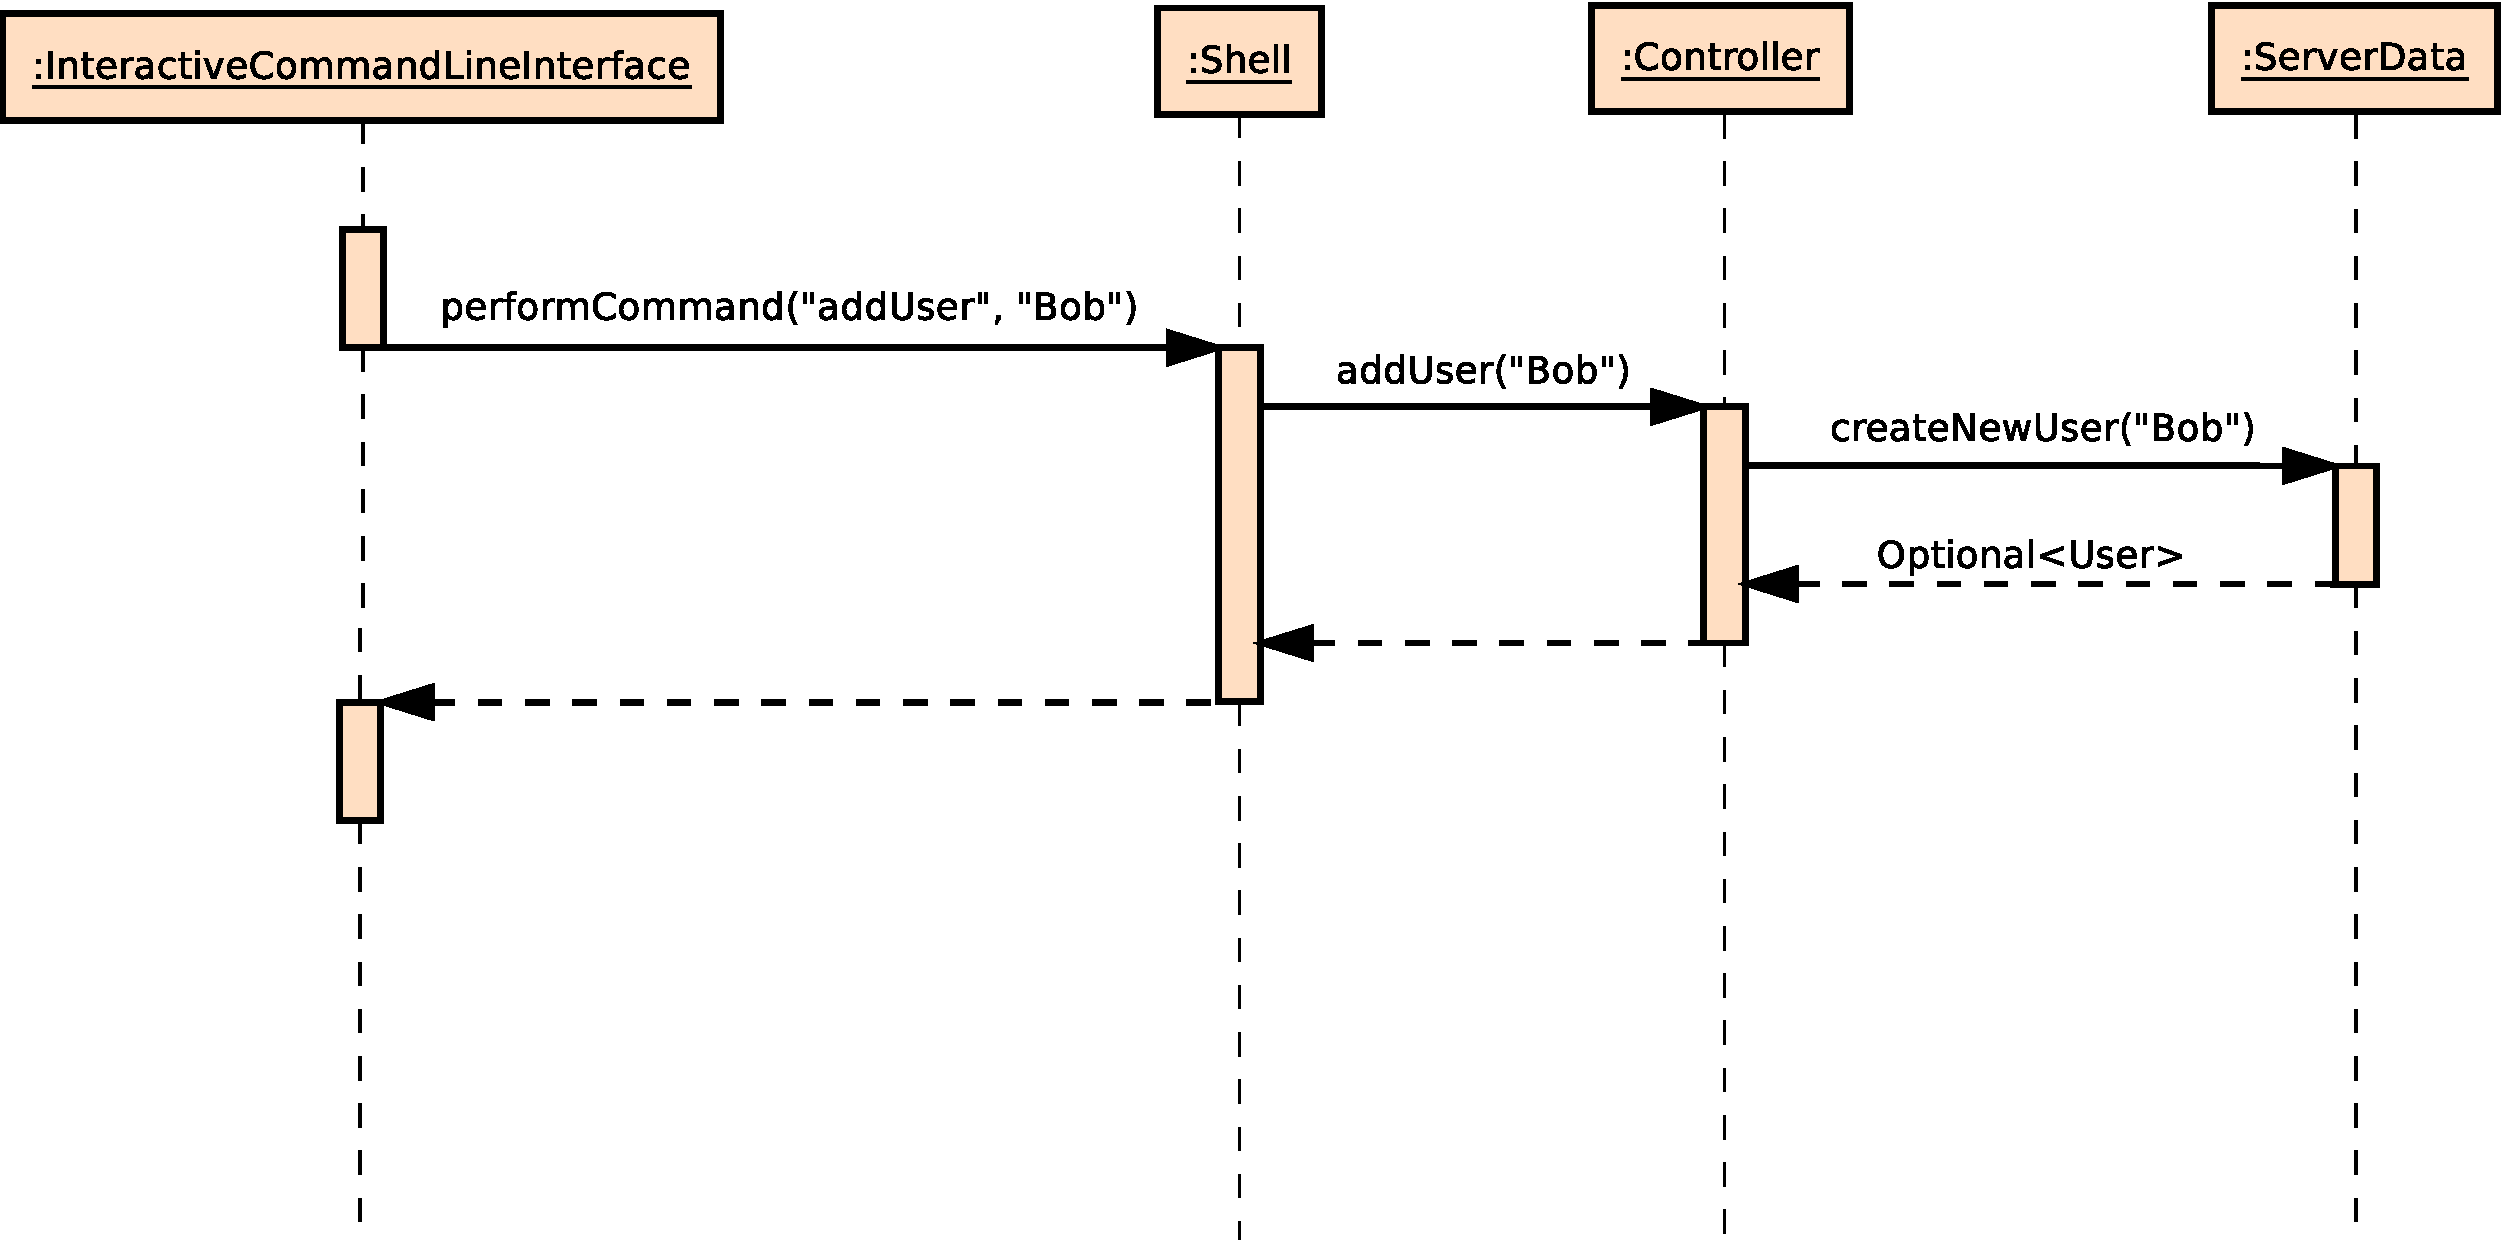
\includegraphics [width=400px] {figures/sequence_diagram_server/Server1.pdf}
\end{illustration}
\begin{illustration}{Sequence diagram of playing a stream for the first time.}
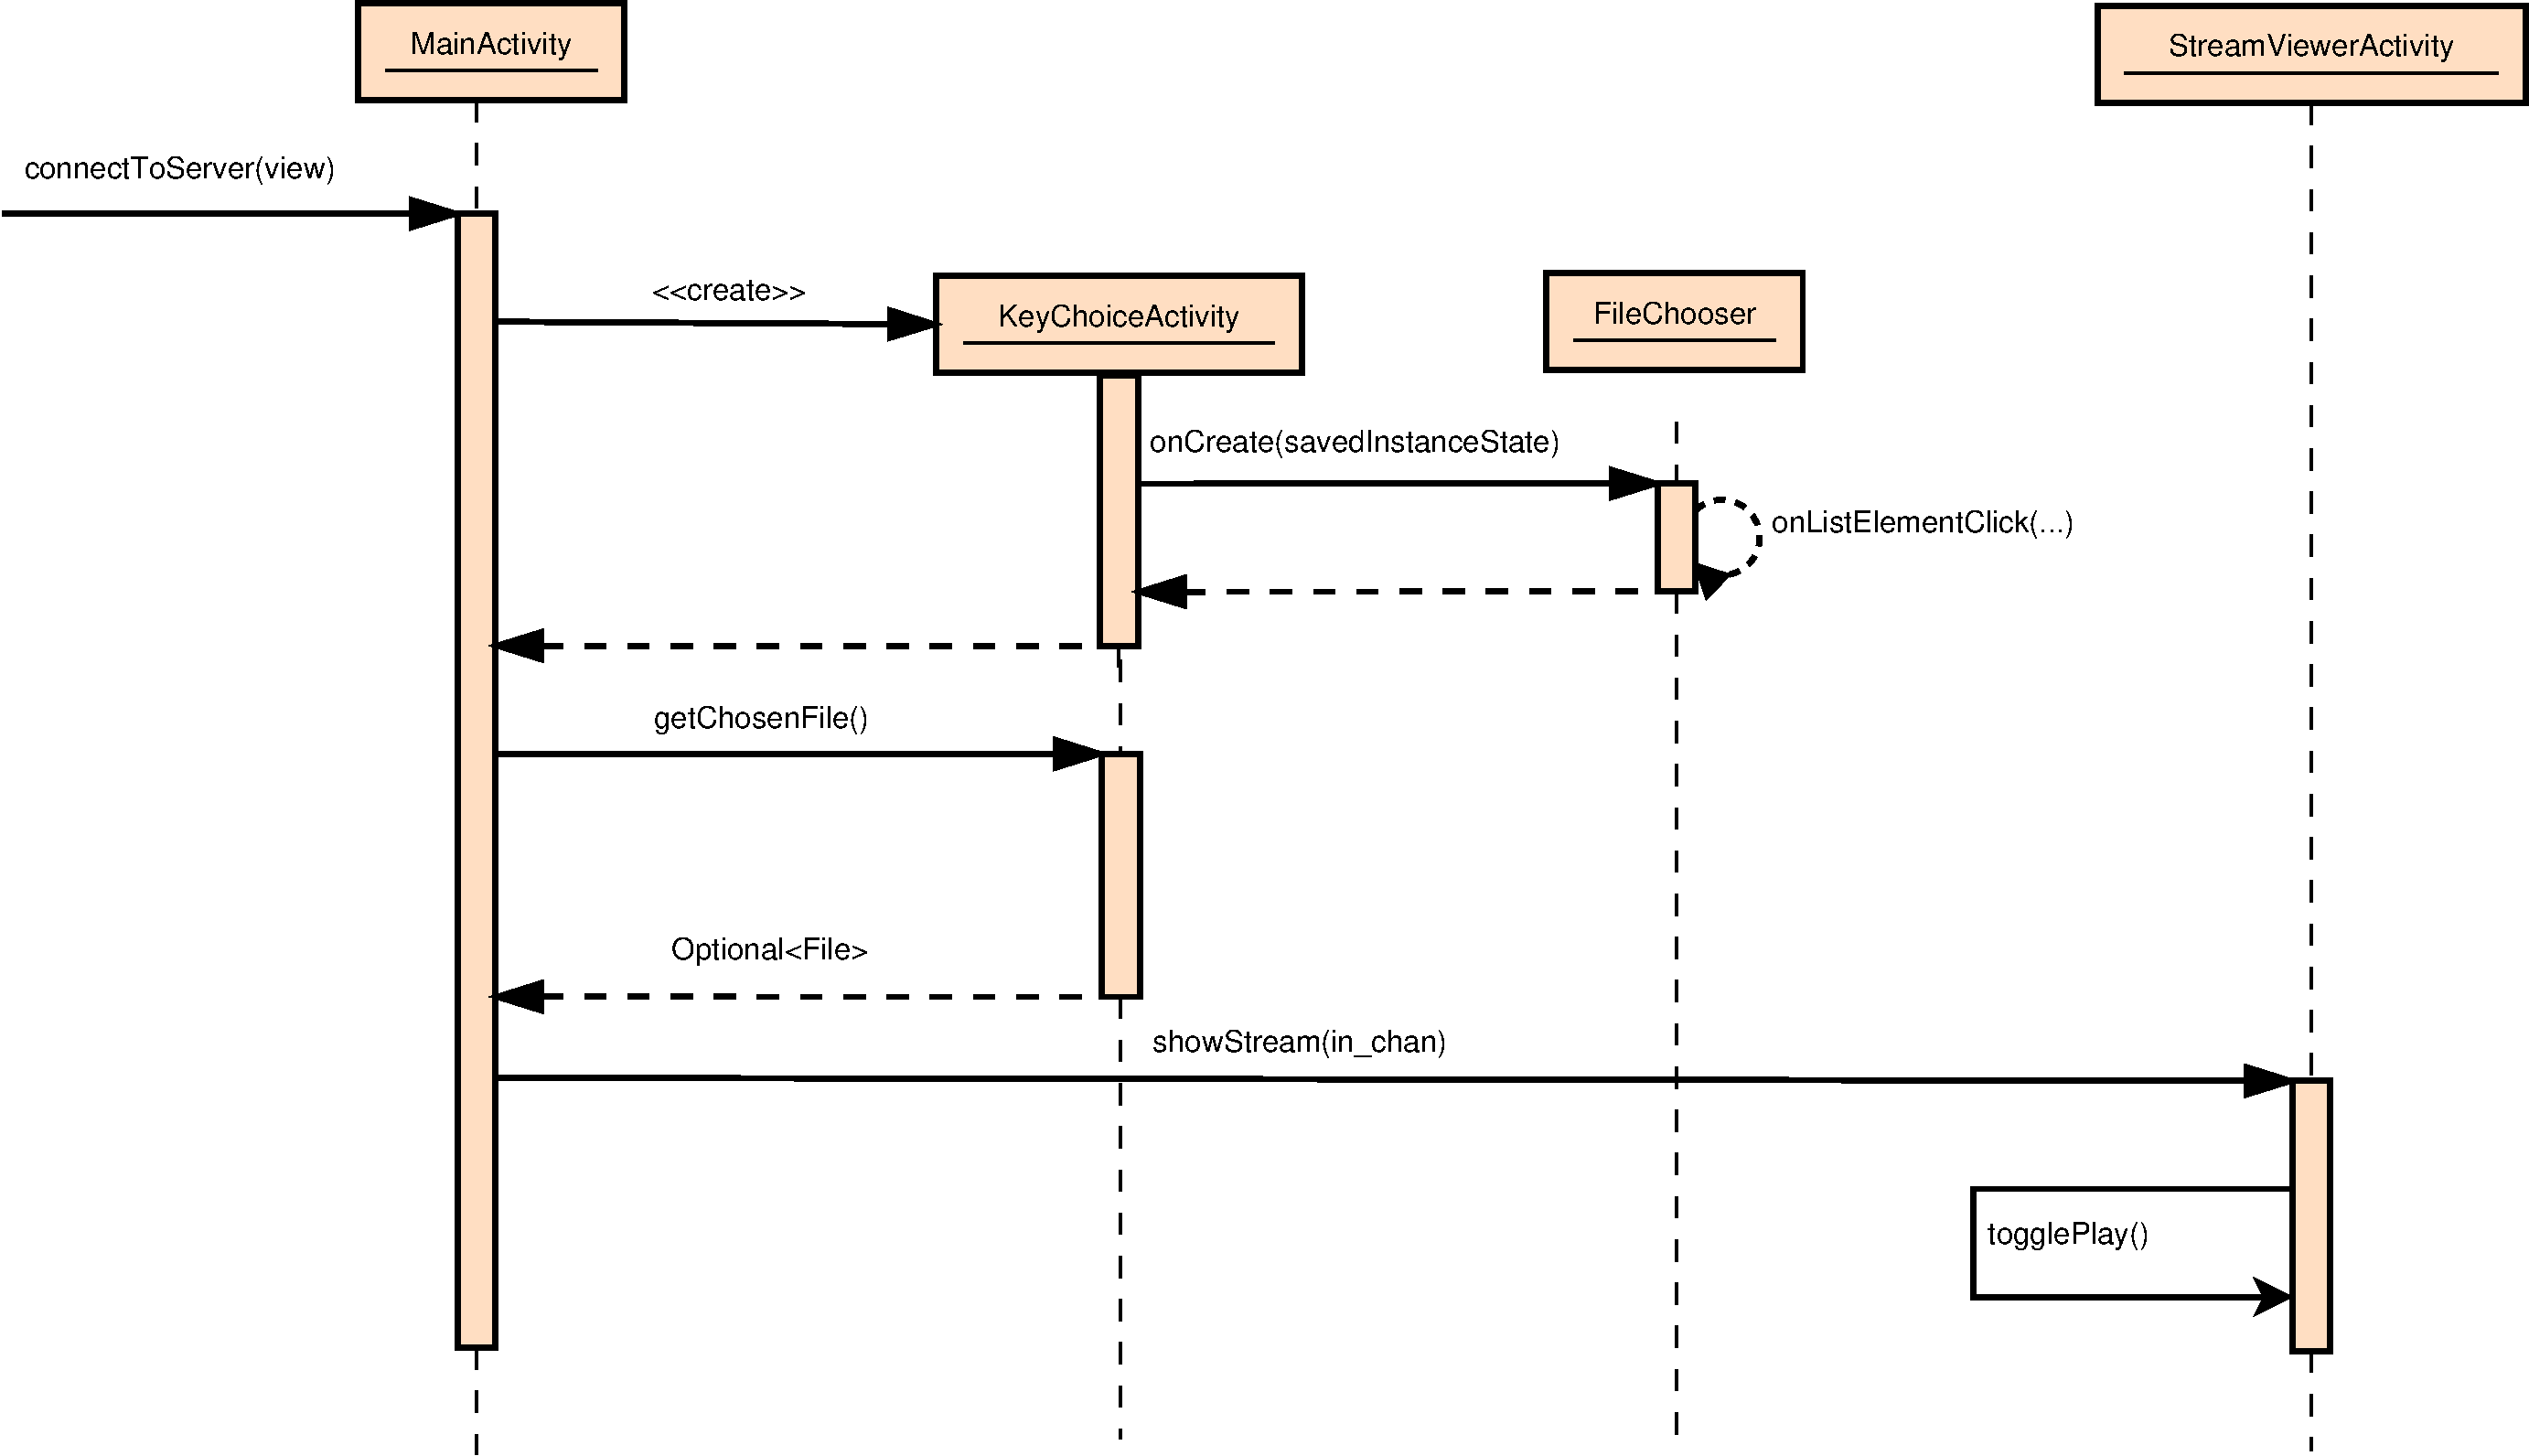
\includegraphics [width=400px] {figures/sequence_diagram_client/sequence_client.pdf}
\end{illustration}

\begin{landscape}
\begin{illustration}{Passing a piece of plaintext data through to the clients (Server side)}
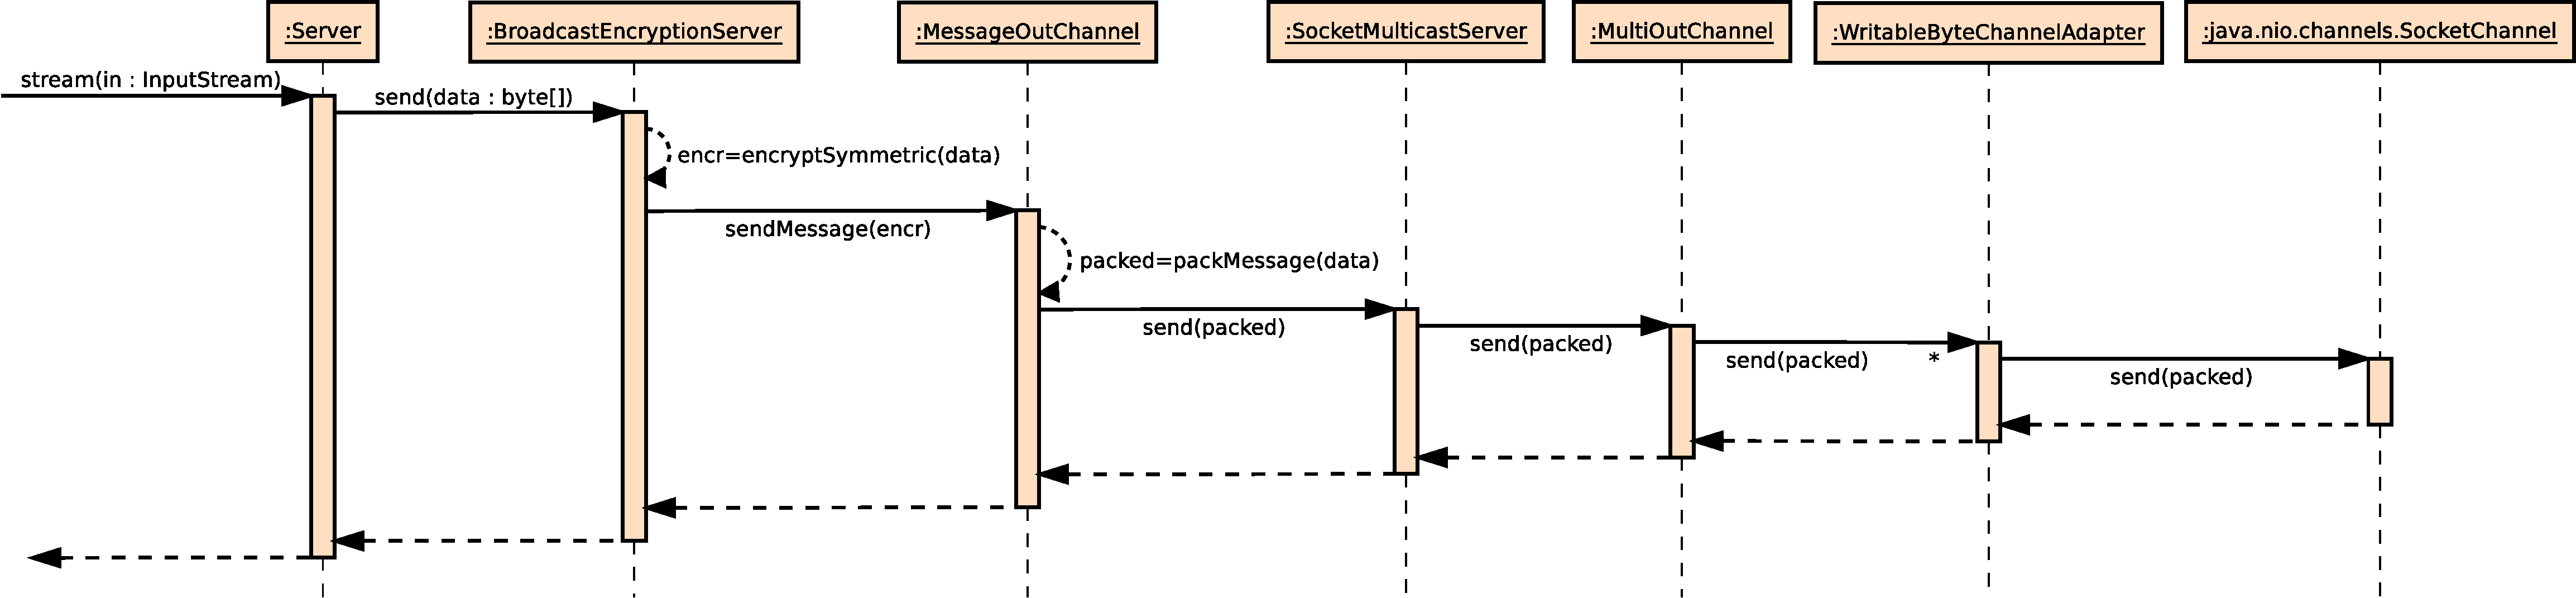
\includegraphics [width=700px] {figures/sequence_diagram_comm1_server/output.pdf}
\end{illustration}
\end{landscape}

\section{GUI design}
The GUI should be user-friendly and intuitional. Therefore its design is very minimalistic, foccusing on its main purpose. 
The following images show prototypes of the graphical user interface.

\begin{illustration}{The main screen which is shown on program start. (The empty space is used for the logo later on))}
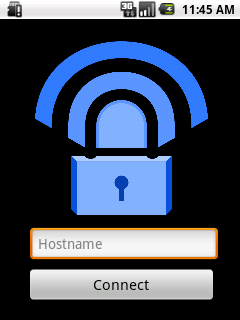
\includegraphics[width=150px]{figures/images/mainscreen.png}
\end{illustration}
\begin{illustration}{The menu which pops up after the menu button is pressed. It allows navigation between the different screens.}
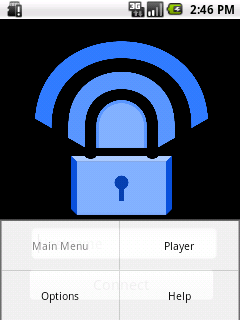
\includegraphics[width=150px]{figures/images/menu.png}
\end{illustration}
\begin{illustration}{The option screen which contains preferences, traffic data and a server history.}
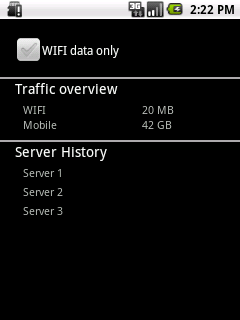
\includegraphics[width=150px]{figures/images/optionscreen.png}
\end{illustration}
\begin{illustration}{An example for an error message.}
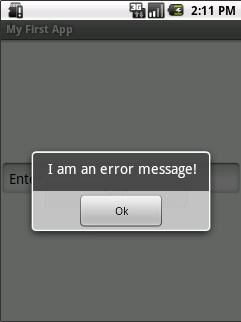
\includegraphics[width=150px]{figures/images/error.png}
\end{illustration}
\begin{illustration}{The file chooser used for selecting a private key.}
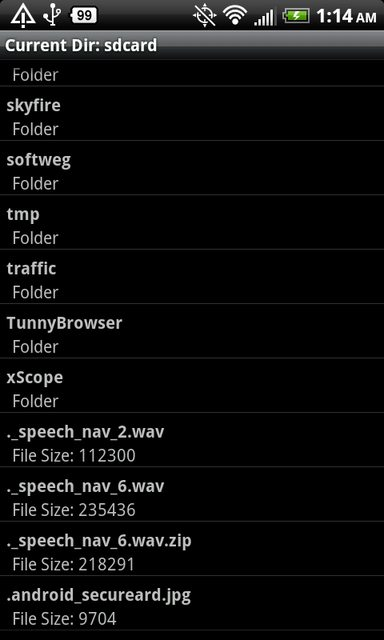
\includegraphics[width=150px]{figures/images/fileChooser.png}
\end{illustration}

\begin{landscape}
\section{Time plan}
   \begin{illustration}{A rough time table for the implementation phase}
  \begin{gantt}[xunitlength=0.5cm,fontsize=\small,titlefontsize=\small,drawledgerline=true]{10}{48}
    \begin{ganttitle}
      \titleelement{2009}{7}
      \numtitle{2010}{1}{2012}{12}
      \titleelement{2013}{5}
    \end{ganttitle}
    \begin{ganttitle}
      \numtitle{6}{1}{12}{1}
      \numtitle{1}{1}{12}{1}
      \numtitle{1}{1}{12}{1}
      \numtitle{1}{1}{12}{1}
      \numtitle{1}{1}{5}{1}
    \end{ganttitle}
    \ganttbar{task 1}{2}{17}
    \ganttgroup{a group of tasks}{6}{18}
    \ganttbar{task 2}{5}{10}
    \ganttbar[pattern=crosshatch,color=blue]{task 3}{15}{3}
    \ganttbar{task 4}{20}{3}
    \ganttcon{15}{4}{20}{6}
    \ganttbar{task 5}{15}{5}
    \ganttbarcon[color=red]{task 6}{20}{5}
    \ganttbarcon{task 7}{30}{5}
  \end{gantt}
  \end{illustration}
\end{landscape}

\end{document}
